\documentclass[12pt]{article}

%%%%% 本文使用的宏包
\usepackage{amsmath}
\usepackage{amsfonts}
\usepackage{mathrsfs}
\usepackage{amssymb}
\usepackage{graphicx} % 插入图形
\usepackage{enumerate}
\usepackage{datetime}
\usepackage{paralist}
\usepackage{color}
\usepackage{float}
\usepackage{nicematrix}
\usepackage{tikz}
\usetikzlibrary{matrix,decorations.pathreplacing}
\usepackage{arydshln}%虚线
\usepackage{algorithm} % 算法
\usepackage{algmatlab}

\usepackage [top=0.8in, bottom=1in, left=2cm, right=2cm]{geometry}

% 其他数学环境
\newtheorem{theorem}{Theorem}[section]
\newtheorem{definition}[theorem]{Definition}
\newtheorem{lemma}[theorem]{Lemma}
\newtheorem{corollary}[theorem]{Corollary}
\newtheorem{proposition}[theorem]{Proposition}
\newtheorem{example}[theorem]{Example}
\newtheorem{remark}[theorem]{Remark}
%\newtheorem{algorithm}[theorem]{Algorithm}

\newenvironment{proof}{\noindent {\bf Proof.\ }}{\vspace{2ex}}

\numberwithin{equation}{section}

%%%%% 参考文件管理
\usepackage{natbib} % 需要作者-年份或高级引用命令
% \usepackage{cite} % 只用数字引用,功能简单
\providecommand{\BIBand}{and}
%%%%%% 引用链接,方便引用跳转可以去掉
\usepackage{hyperref}
\hypersetup{
colorlinks=true, 
citecolor=blue,
linkcolor=black}
%%%%%% 

\usepackage{cleveref} % 智能引用

\usepackage{caption} % 用于设置标题格式
% 设置图片标题前缀为 "Fig."
\captionsetup[figure]{name=Figure}5
\captionsetup[algorithm]{name=Algorithm}

% 设置 cleveref 引用前缀4
\crefname{figure}{Fig.}{Figs.} % 单数/复数形式
\crefname{algorithm}{Algorithm}{Algorithms} % 单数/复数形式

%%%% 编辑临时使用
\newcommand{\red}{\color{red}}

% 重定义摘要环境的标题样式
\makeatletter
\renewenvironment{abstract}{%
  % \small
  % \begin{center}% 注释掉这行可取消默认居中
  \noindent\bfseries \abstractname \par%
  \normalfont
  % \end{center}% 注释掉这行可取消默认居中
  % \vspace{-.5em}\noindent\rule{\textwidth}{0.4pt}\vspace{.5em}% 可选:添加下划线
  \list{}{%
    \leftmargin=0cm% 左边距为0
    \rightmargin=0cm% 右边距为0
  }%
  \item\relax
}{%
  \endlist
}
\makeatother

\newcommand\blfootnote[1]{%
  \begingroup
  \renewcommand\thefootnote{}\footnote{#1}%
  \addtocounter{footnote}{-1}%
  \endgroup
}

\begin{document}

%-------------------- FRONTMATTER --------------------
\begin{center}

% 标题
{\LARGE \textbf{An Algorithm for QR Decomposition of Split Quaternion Matrices} }

\blfootnote{This research is supported by Macao Science and Technology Development Fund (No. 0013/2021/ITP), the grants from the National Natural Science Foundation of China  (12371023, 12271338, 12001259), and the Natural Sciences and Engineering Research Council of Canada (NSERC) (RGPIN 2020-06746), The Joint Research and Development Fund of Wuyi University, Hong Kong and Macao (2019WGALH20), The MUST Faculty Research Grants (FRG-22-073-FIE). \par
* Corresponding author
E-mail: xiliu@must.edu.mo
 }
%作者与机构 
\bigskip
$${\textbf{Qianqian Liu}^{1}, \textbf{Xin Liu}^{2, \ast}, \textbf{Jianhai Lin}^{3}, \textbf{Yang Zhang}^{4}}$$
\newline $^{\text{1,3}}$Faculty of Innovation Engineering, Macau University of Science and Technology, Avenida Wai Long, TaiPa, Macau, 999078, China; 
\newline $^{\text{2}}$Macau Institute of Systems Engineering, Faculty of Innovation Engineering, Macau University of Science and Technology, Avenida Wai Long, TaiPa, Macau, 999078, China;
% \newline $^{\text{3}}$Faculty of Innovation Engineering, Macau University of Science and Technology, Avenida Wai Long, TaiPa, Macau, 999078, China;
\newline $^{\text{4}}$ Department of Mathematics, University of Manitoba, Winnipeg, MB, R3T 2N2, Canada. \\
\bigskip
\end{center}

% 摘要

\begin{abstract}
Split quaternion algebra is not a Euclidean distance space because of having zero divisors. Thus, the traditional QR decomposition based on Givens rotations and Householder reflection transformations is difficult to implement. To overcome this difficulty and to address the non-commutativity of split quaternion multiplication, we utilize the real representation $A^\sigma$ of the split quaternion matrix $A$. By leveraging the proposed decomposition $A^\sigma = \widetilde{Q}R_4$ ($\widetilde{Q}$ is an orthogonal matrix, and $R_4 = \begin{bmatrix} R_{11} & R_{12} \\ R_{21} & R_{22} \end{bmatrix}$ with $R_{11}, R_{12}, R_{21}, R_{22}$ being upper triangular), the QR decomposition of $A$ is successfully constructed and the corresponding algorithms are developed.The experimental results show that it performs well in both speed and accuracy.
\end{abstract}
%关键词
\noindent\textbf{Keywords} Split quaternion matrix, QR decomposition, Permutation matrix, Upper triangular matrix
\\
\noindent\textbf{AMS 2010 Subject Classification:} 15B10, 15B33, 15A20, 15A23.

%-------------------- 正文主体 --------------------

\section{Introduction}
In 1849, James Cockle \citep{Cockle1849} introduced the concept of split quaternion algebra over the real number field $\mathbb{R}$, which is defined as:
\begin{equation*}
    \mathbb{H}_s = \left\{ a_0 + a_1 i + a_2 j + a_3 k \ \bigg| \ i^2 = -1,\ j^2 = k^2 = 1, \ ijk = 1, \ a_0, a_1, a_2, a_3 \in \mathbb{R}\right\}. 
\end{equation*} 

 $\mathbb{H}_s$ is a four dimensional non-commutative algebra and contains zero divisors. 
  In the past decades, many studies have been done on the \iffalse algebraic properties of \fi split quaternions \citep{AR2020,Yasemin2012,TJiang2015,Jiang2018,TJiang2018,Zhuo2020,Yang2020,mma2023,wang2024,Wang2021,Gang2024,yuan2017,Zhang2015} and  many applications have been found in quantum mechanics, electromagnetism, signal processing, etc. \citep{Gog2022, Hasebe2010, Z2022, Wang2023}. For instance, \citep{Jiang2018} studied the eigenvalue problem of split quaternion matrices; \iffalse \cite{Xin2019} derived a new real representation of split quaternion matrices to explain the consistency of two types of split quaternion matrix equations \(AX^* - XB = CY + D\) and \(X - AX^*B = CY + D\); \fi \citep{wang2024} solved a classical system of matrix equations; 
 \citep{Wang2021} proposed a fast algorithm for LDU decomposition; \citep{Gang2024} developed an efficient algorithm for the SVD. However, existing research has not yet fully addressed the theoretical development and algorithmic implementation of QR decomposition for split quaternion matrices.
 
We acknowledge that the split quaternion algebra does not constitute an Euclidean space, rendering traditional Givens rotations and Householder reflections inapplicable when applied to split quaternion vectors. This poses a substantial challenge for the conventional QR decomposition process for split quaternion matrices.

To address the above problem, we intend to utilize the real representation of split quaternions. Indeed, there exist multiple forms of such real representations \citep{Zhuo2020, Yang2020, Xin2019, Gang2024}. For example,  a split quaternion matrix $A$ of size $m \times n$  can be represented as a real matrix $A^\sigma$ 
  with dimensions $4m \times 4n$ \citep{Xin2019}. In contrast, the real representation matrix presented in \cite{Gang2024} has a dimension of $2m \times 2n$. Compared to the former, the $2m \times 2n$ real representation matrix offers more advantages in terms of dimension expansion. By employing this compact real representation, the  problem of split quaternion decomposition is converted into a specific decomposition problem for real matrices. This approach not only presents the potential for reducing computational time but also streamlines the algorithm's complexity. Therefore, through the use of the real representation method, 
we constructively prove the existence of QR decomposition for split quaternion matrices and propose a novel and efficient algorithm for its computation. To validate the high efficiency of our algorithm, we provide the experimental results in terms of speed and accuracy.

The paper is organized as follows. In Section 2, the real representation of split quaternion matrices and their properties are introduced. In Section 3, a constructive proof of the existence of QR decomposition for split quaternion matrices is provided, along with the corresponding algorithm and an analysis of its computational complexity. In Section 4, we use one example to show the efficiency and accuracy of our algorithm. We also use another example to show the application in solving a split quaternion matrix equation. Finally, the contributions of this paper and future work are summarized in Section 5.


\section{Preliminaries}
For any split quaternion matrix ${A}=A_{0}+A_{1}i + A_{2}j + A_{3}k \in\mathbb{H}_{s}^{m\times n}$, where $A_{i}\in\mathbb{R}^{m\times n}, i\in\{0,1,2,3\}$, its transpose, conjugate, conjugate transpose, i-conjugate and i-conjugate transpose are  denoted by 
 ${A}^T = A_0^T + A_1^Ti + A_2^Tj + A_3^Tk, \ \bar{{A}} = A_0 - A_1i - A_2j - A_3k, \ {A}^* = A_0^T - A_1^Ti - A_2^Tj - A_3^Tk,$ and
 $\tilde{A} = A_0 - A_1i + A_2j + A_3k, \ {A}^H = A_0^T - A_1^Ti + A_2^Tj + A_3^Tk$, respectively. Recall that the real representation matrix of a split quaternion matrix $A \in\mathbb{H}_{s}^{m\times n}$ can be presented as \citep{TJiang2018, Gang2024}:
\begin{equation}\label{eq:2.1}
A^\sigma = \begin{bmatrix} A_0 + A_2 & -A_1 + A_3 \\ A_1 + A_3 & A_0 - A_2 \end{bmatrix} \in \mathbb{R}^{2m \times 2n}.
\end{equation}

For $A, B \in \mathbb{H}_s^{m \times n}$, $C \in \mathbb{H}_s^{n \times p}$, $a \in \mathbb{R}$, the following properties hold:
\begin{equation}\label{eq:2.2}
    (A + B)^\sigma = A^\sigma + B^\sigma, \quad (AC)^\sigma = A^\sigma C^\sigma, \quad (a A)^\sigma = a A^\sigma, \ (A^H)^\sigma = (A^\sigma)^T.
\end{equation}
Conversely, for any real matrix $B = \begin{bmatrix} B_{11} & B_{12} \\ B_{21} & B_{22} \end{bmatrix} \in \mathbb{R}^{2m \times 2n}$, $B_{ts} \in \mathbb{R}^{m \times n}$, $t, s = 1, 2$, a corresponding split quaternion matrix $A$ can be constructed as follows:
\begin{equation}\label{eq:2.3}
{A} = \frac{B_{11} + B_{22}}{2} + \frac{B_{21} - B_{12}}{2}i + \frac{B_{11} - B_{22}}{2}j + \frac{B_{21} + B_{12}}{2}k.
\end{equation}

From equation \eqref{eq:2.1}, we have ${A}^\sigma = B$. 
That is, $\sigma$ provides an one-to-one corresponding between $\mathbb{H}_s^{m\times n}$ and $\mathbb{R}^{2m \times 2n}$ \citep{Gang2024}. Furthermore, $A$ is called unitary if $AA^H = A^H A = I$. $A$ is unitary if and only if $A^\sigma$ is orthogonal.
 The Frobenius norm of $A$ is defined as: 
 \begin{align*}
 % $
     \| A \|_F \equiv \frac{1}{\sqrt{2}} \| A^\sigma \|_F = \sqrt{\| A_0 \|_F^2 + \| A_1 \|_F^2 + \| A_2 \|_F^2 + \| A_3 \|_F^2}.
% $
\end{align*}
\iffalse 
When $U$ and $ V$ are unitary, $U^\sigma$ and $V^\sigma$ are orthogonal, {\color{red} which will not change the Frobenius norm of $A^\sigma$. Hence, ???}\fi
If $U$ and $ V$ are unitary, then $U^\sigma$ and $V^\sigma$ are orthogonal.  Hence,
\begin{align*}
 % $
\|UAV\|_F = \frac{1}{\sqrt{2}} \|(UAV)^\sigma\|_F 
= \frac{1}{\sqrt{2}} \|U^\sigma A^\sigma V^\sigma\|_F 
= \frac{1}{\sqrt{2}} \|A^\sigma\|_F 
= \|A\|_F.
 % $
\end{align*}

\section{QR Decomposition of Split Quaternion Matrices}
In this section, we discuss the QR decomposition of split quaternion matrices through construction, and develop an efficient algorithm for computing it. Let $A \in \mathbb{H}_s^{m \times n}$, we will achieve this through a two-step process.

\noindent \textbf{Step 1:} To construct the upper triangular split quaternion matrix, we will apply row/column transformations to rewrite the QR decomposition of $A^\sigma \in \mathbb{R}^{2m \times 2n}$ as 
\begin{equation}\label{splitqr}
A^\sigma = \widetilde{Q} R_4,
\end{equation} 
where $\widetilde{Q} \in \mathbb{R}^{2m\times 2m}$ is orthogonal, and $R_4$ is in the form of 
\begin{equation}\label{r4}
R_4 = \begin{bmatrix}
    R_{11} & R_{12} \\
    R_{21} & R_{22}
\end{bmatrix} \in \mathbb{R}^{2m \times 2n},
\end{equation}
and $R_{11}, R_{12},R_{21},R_{22}$ are all upper triangular matrices of size $m \times n$. This is the challenge part of our paper, and only this special decomposition accomplished, then we can subsequently construct the corresponding unitary matrix \(Q\) and upper triangular matrix \(R\) for the QR decomposition of \(A\).

To achieve the special decomposition \eqref{splitqr}, we first figure out how to transform an upper triangular matrix $R$ into $R_4$ (\cref{fig:Figure_1}) through permutation transformations:
\iffalse
For a given matrix $R\in \mathbb{R}^{2m \times 2n}$, we swap its rows $r_i$ as follows: 
\begin{equation}\label{rowswap}
r_2\longleftrightarrow r_{m +1 + (m \bmod 2)}, \ \  r_4\longleftrightarrow r_{m+3+(m \bmod 2)}, \ \dots, \ \   r_{m - (m \bmod 2)}   \longleftrightarrow r_{2m-1}.
\end{equation}
{\color{red} Above formulas do not match the precess of example???}

Next we partition the resulting matrix into the upper matrix $R_{upper}\in \mathbb{R}^{m \times 2n}$ and the lower matrix $R_{lower}\in \mathbb{R}^{m \times 2n}$. If $m$ is odd, appending a zero row to the end of the last row of the upper submatrix and prepending a zero row to the beginning of the first row of the lower submatrix ensure that the parity of each row index remains unchanged before the swap, the position of a zero row stays fixed after the swap, and further partitioning is possible. The next is removing the added zero rows to keep the same size. Subsequently, for  $R_{upper}$ and $ R_{lower}$, recursively apply the aforementioned row swapping and partitioning, zero-padding, and zero-removing operations to each submatrix until each submatrix contains only two rows. Analogous operations are performed on the columns, ultimately producing the resulting matrix $R_4$.
It is the key to accomplishing the special decomposition \eqref{splitqr}.
\fi
\newline
\newline
First, perform row permutations on $R\in \mathbb{R}^{2m \times 2n}$:
\begin{enumerate}
\item Swap its rows $r_i$ as follows:  
   \begin{equation} \label{eq:rowswap}
       r_2 \leftrightarrow r_{m + 1 + (m \bmod 2)}, \quad r_4 \leftrightarrow r_{m + 3 + (m \bmod 2)}, \quad \dots, \quad r_{m - (m \bmod 2)} \leftrightarrow r_{2m - 1}.
   \end{equation}
\item  Partition the swapped matrix into an upper submatrix \( R_{\text{upper}} \in \mathbb{R}^{m \times 2n} \) and a lower submatrix \( R_{\text{lower}} \in \mathbb{R}^{m \times 2n} \). If \( m \) is odd, append a zero row to the end of the last row of \( R_{\text{upper}} \) and prepend a zero row to the beginning of the first row of \( R_{\text{lower}} \) ensuring that the parity of each row index remains unchanged before the swap, the position of the zero row stays fixed after the swap, and further partitioning is possible.
 
\item Repeat steps 1 and 2 for \( R_{\text{upper}} \) and \( R_{\text{lower}} \) until all  partitioned submatrices contain exactly 2 rows.  
 
\item  Remove the added zero rows in step 2 to keep the same size.
\end{enumerate}
Second, proceed to perform column permutations on resulting matrix:
\begin{enumerate}
\item For the columns \( c_i \) of the resulting matrix, we swap as follows:  
   \begin{equation} \label{eq:cswap}
       c_2 \leftrightarrow c_{n + 1 + (n \bmod 2)}, \quad c_4 \leftrightarrow c_{n + 3 + (n \bmod 2)}, \quad \dots, \quad c_{n - (n \bmod 2)} \leftrightarrow c_{2n - 1}.
   \end{equation}  
\item  Partition the swapped matrix into a left submatrix \( R_{\text{left}} \in \mathbb{R}^{2m \times n} \)  and a right submatrix \( R_{\text{right}} \in \mathbb{R}^{2m \times n} \). If \( n \) is odd, append a zero column to the end of the last column of \( R_{\text{left}} \) and prepend a zero column to the beginning of the first column of \( R_{\text{right}} \), ensuring that the parity of each column index remains unchanged before the swap, the position of the zero column stays fixed after the swap, and further partitioning is possible.  
 
\item  Repeat steps 1 and 2 for \( R_{\text{left}} \) and \( R_{\text{right}} \) until all partitioned submatrices contain exactly 2 columns. 
 
\item Remove the added zero columns in step 2 to keep the same size.
\end{enumerate}


 Ultimately, the matrix \( R_4 \) is obtained through the above row and column permutations.

\begin{figure}[htbp]
    % \begin{minipage}[htbp]{0.45\textwidth}
        \centering
        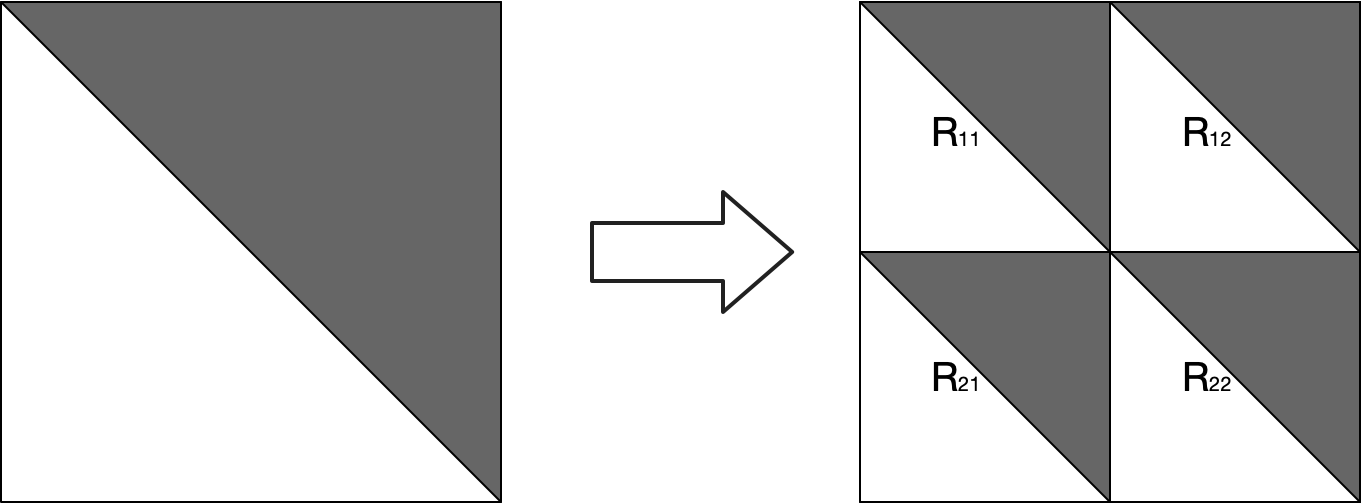
\includegraphics[width=0.45\textwidth,keepaspectratio=true]{Figure_1.png} % Replace with actual file name
        \caption{From $R$ to $R_4$ by permutations }
        \label{fig:Figure_1}
\end{figure}


\iffalse
{\color{red}V1: Perform swaps on the rows of $R\in \mathbb{R}^{2m \times 2n}$: $r_2\leftrightarrow r_{m +1 + (m \bmod 2)}$, $r_4\leftrightarrow r_{m+3+(m \bmod 2)}$, $\dots$, $r_{m - (m \bmod 2)} \leftrightarrow r_{2m-1}$. Then partition the resulting matrix into  the upper matrix $R_{upper}\in \mathbb{R}^{m \times 2n}$ and the lower matrix $R_{lower}\in \mathbb{R}^{m \times 2n}.$ If $m$ is odd, appending zeros row to the end of the last row of the upper submatrix and prepending zeros row to the beginning of the first row of the lower submatrix ensures that the parity of each row index remains unchanged before the swap, the position of zero rows stays fixed after the swap, and further partitioning is possible. The next is removing the added zeros rows to keep the same size. Subsequently, for the $R_{upper}, R_{lower}$, recursively apply the aforesaid row swapping and partitioning, zero-padding and zero-removing operations to each submatrix until each submatrix contains only two rows; analogous operations are performed on the columns, ultimately yielding the resulting matrix $R_4$.}
\fi 
To better understand the procedure, we choose the following matrix 
\[R= \begin{bmatrix}
 r_{11} & r_{12} & r_{13} & r_{14} & r_{15} & r_{16} & r_{17} & r_{18}\\
 0      & r_{22} & r_{23} & r_{24} & r_{25} & r_{26} & r_{27} & r_{28}\\
 0      & 0      & r_{33} & r_{34} & r_{35} & r_{36} & r_{37} & r_{38}\\
 0      & 0      & 0      & r_{44} & r_{45} & r_{46} & r_{47} & r_{48}\\
 0      & 0      & 0      & 0      & r_{55} & r_{56} & r_{57} & r_{58}\\
 0      & 0      & 0      & 0      & 0      & r_{66} & r_{67} & r_{68}\\
\end{bmatrix} \in \mathbb{R}^{2\cdot 3 \times 2 \cdot 4}
\]
to show how the row/column transformations work. 
\iffalse
Through the above process, we have
\iffalse

show how our method works.  We will first describe how to achieve this in the algorithm, followed by providing the theoretical underpinning for the operation:
\fi

  \iffalse Perform swaps on the rows of $R\in \mathbb{R}^{2m \times 2n}$: $r_2\leftrightarrow r_{m +1 + (m \bmod 2)}$, $r_4\leftrightarrow r_{m+3+(m \bmod 2)}$, $\dots$, $r_{m - (m \bmod 2)}$ $ \leftrightarrow r_{2m-1}$. Then partition the resulting matrix into the upper matrix $R_{upper}\in \mathbb{R}^{m \times 2n}$ and the lower matrix $R_{lower}\in \mathbb{R}^{m \times 2n}.$ If $m$ is odd, appending zeros row to the end of the last row of the upper submatrix and prepending zeros row to the beginning of the first row of the lower submatrix ensures that the parity of each row index remains unchanged before the swap, the position of zero rows stays fixed after the swap, and further partitioning is possible. The next is removing the added zeros rows to keep the same size. Subsequently, for the $R_{upper}, R_{lower}$, recursively apply the aforesaid row swapping and partitioning, zero-padding and zero-removing operations to each submatrix until each submatrix contains only two rows; analogous operations are performed on the columns, ultimately yielding the resulting matrix $R_4$.  This corresponding process can be realized by Algorithm \cref{alg:Permutation}. In this way, we can obtain\fi
\iffalse
\[R = \begin{bmatrix}
\begin{array}{cccc:cccc}
 r_{11} & r_{13} & r_{15} & r_{17} & r_{12} & r_{14} & r_{16} & r_{18}\\
 0      & r_{33} & r_{35} & r_{37} & 0      & r_{34} & r_{36} & r_{38}\\
 0      & 0      & r_{55} & r_{57} & 0      & 0      & r_{56} & r_{58}\\
 \cdashline{1-8}
 0      & r_{23} & r_{25} & r_{27} & r_{22} & r_{24} & r_{26} & r_{28}\\
 0      & 0      & r_{45} & r_{47} & 0      & r_{44} & r_{46} & r_{48}\\
 0      & 0      & 0      & r_{67} & 0      & 0      & r_{66} & r_{68}\\
\end{array}
\end{bmatrix}=\begin{bmatrix}
    R_{11} & R_{12}\\R_{21} & R_{22}
\end{bmatrix}.\]
\fi

\begin{align*}
R &=
  \begin{bmatrix}
 r_{11} & r_{12} & r_{13} & r_{14} & r_{15} & r_{16} & r_{17} & r_{18}\\
 0      & r_{22} & r_{23} & r_{24} & r_{25} & r_{26} & r_{27} & r_{28}\\
 0      & 0      & r_{33} & r_{34} & r_{35} & r_{36} & r_{37} & r_{38}\\
 0      & 0      & 0      & r_{44} & r_{45} & r_{46} & r_{47} & r_{48}\\
 0      & 0      & 0      & 0      & r_{55} & r_{56} & r_{57} & r_{58}\\
 0      & 0      & 0      & 0      & 0      & r_{66} & r_{67} & r_{68}\\
\end{bmatrix}
\xrightarrow{r_{2} \leftrightarrow r_{5}}
\begin{bmatrix}
% \begin{array}{cc:cc:cc}
 r_{11} & r_{12} & r_{13} & r_{14} & r_{15} & r_{16} & r_{17} & r_{18}\\
 0      & 0      & 0      & 0      & r_{55} & r_{56} & r_{57} & r_{58}\\
 0      & 0      & r_{33} & r_{34} & r_{35} & r_{36} & r_{37} & r_{38}\\
 % \cdashline{1-8}
 0      & 0      & 0      & r_{44} & r_{45} & r_{46} & r_{47} & r_{48}\\
 0      & r_{22} & r_{23} & r_{24} & r_{25} & r_{26} & r_{27} & r_{28}\\
 0      & 0      & 0      & 0      & 0      & r_{66} & r_{67} & r_{68}\\
% \end{array}
\end{bmatrix}.
\end{align*}\\
Next, partition the matrix into \( R_{upper} \) and \( R_{lower} \). Due to the fact that both \( R_{upper} \) and \( R_{lower} \) have an odd number of rows, we must append a zero row to the end of the last row of \( R_{upper} \) and prepend a zero row to the beginning of the first row of \( R_{lower} \): \begin{align*}
& \begin{bmatrix}
 r_{11} & r_{12} & r_{13} & r_{14} & r_{15} & r_{16} & r_{17} & r_{18}\\
 0      & 0      & 0      & 0      & r_{55} & r_{56} & r_{57} & r_{58}\\
 0      & 0      & r_{33} & r_{34} & r_{35} & r_{36} & r_{37} & r_{38}\\
 \cdashline{1-8}
 0      & 0      & 0      & r_{44} & r_{45} & r_{46} & r_{47} & r_{48}\\
 0      & r_{22}  & r_{23} & r_{24} & r_{25} & r_{26} & r_{27} & r_{28}\\
 0      & 0      & 0      & 0      & 0      & r_{66} & r_{67} & r_{68}\\
\end{bmatrix}
\xrightarrow{add\ zero\ rows}
\begin{bmatrix}
 r_{11} & r_{12} & r_{13} & r_{14} & r_{15} & r_{16} & r_{17} & r_{18}\\
 0      & 0      & 0      & 0      & r_{55} & r_{56} & r_{57} & r_{58}\\
 0      & 0      & r_{33} & r_{34} & r_{35} & r_{36} & r_{37} & r_{38}\\
 0      & 0      & 0      & 0      & 0      & 0      & 0      & 0     \\
 \cdashline{1-8}
 0      & 0      & 0      & 0      & 0      & 0      & 0      & 0     \\
 0      & 0      & 0      & r_{44} & r_{45} & r_{46} & r_{47} & r_{48}\\
 0      & r_{22} & r_{23} & r_{24} & r_{25} & r_{26} & r_{27} & r_{28}\\
 0      & 0      & 0      & 0      & 0      & r_{66} & r_{67} & r_{68}\\
\end{bmatrix} 
\end{align*}
Next, we proceed by performing row swaps on both \( R_{upper} \) and \( R_{lower} \) individually, following \eqref{rowswap}. Afterward, we eliminate the zero rows that were added in order to maintain the original dimensions of the matrices:\\
% &\xrightarrow{partition\ to\ R_{upper},\ R_{lower}}
\begin{align*}
\xrightarrow[r_{2} \leftrightarrow r_{3}\ in\ R_{lower}]{r_{2} \leftrightarrow r_{3}\ in\ R_{upper}}
&\begin{bmatrix}
 r_{11} & r_{12} & r_{13} & r_{14} & r_{15} & r_{16} & r_{17} & r_{18}\\
 0      & 0      & r_{33} & r_{34} & r_{35} & r_{36} & r_{37} & r_{38}\\
 0      & 0      & 0      & 0      & r_{55} & r_{56} & r_{57} & r_{58}\\
 0      & 0      & 0      & 0      & 0      & 0      &  0     & 0     \\
\cdashline{1-8}
 0      & 0      & 0      & 0      & 0      & 0      & 0      & 0     \\
 0      & r_{22} & r_{23} & r_{24} & r_{25} & r_{26} & r_{27} & r_{28}\\
 0      & 0      & 0      & r_{44} & r_{45} & r_{46} & r_{47} & r_{48}\\
 0      & 0      & 0      & 0      & 0      & r_{66} & r_{67} & r_{68}\\
\end{bmatrix}\\
\xrightarrow{remove\ zero\ rows}
&\begin{bmatrix}
 r_{11} & r_{12} & r_{13} & r_{14} & r_{15} & r_{16} & r_{17} & r_{18}\\
 0      & 0      & r_{33} & r_{34} & r_{35} & r_{36} & r_{37} & r_{38}\\
 0      & 0      & 0      & 0      & r_{55} & r_{56} & r_{57} & r_{58}\\
 0      & r_{22} & r_{23} & r_{24} & r_{25} & r_{26} & r_{27} & r_{28}\\
 0      & 0      & 0      & r_{44} & r_{45} & r_{46} & r_{47} & r_{48}\\
 0      & 0      & 0      & 0      & 0      & r_{66} & r_{67} & r_{68}\\
\end{bmatrix}
\end{align*}
Now we perform column swaps \begin{equation}\label{cswap}
c_2\longleftrightarrow c_{n +1 + (n \bmod 2)}, \ \  c_4\longleftrightarrow c_{n+3+(n \bmod 2)}, \ \dots, \ \   c_{n - (n \bmod 2)}   \longleftrightarrow c_{2n-1}.
\end{equation}
\begin{align*}
\xrightarrow{c_{2} \leftrightarrow c_{5}}
&\begin{bmatrix}
 r_{11} & r_{15} & r_{13} & r_{14} &  r_{12} & r_{16} & r_{17} & r_{18}\\
 0      & r_{35} & r_{33} & r_{34} &  0      & r_{36} & r_{37} & r_{38}\\
 0      & r_{55} & 0      & 0      &  0      & r_{56} & r_{57} & r_{58}\\
 0      & r_{25} & r_{23} & r_{24} &  r_{22} & r_{26} & r_{27} & r_{28}\\
 0      & r_{45} & 0      & r_{44} &  0      & r_{46} & r_{47} & r_{48}\\
 0      & 0      & 0      & 0      &  0      & r_{66} & r_{67} & r_{68}\\
\end{bmatrix}
\end{align*}
\begin{align*}
\xrightarrow{c_{4} \leftrightarrow c_{7}}
&\begin{bmatrix}
 r_{11} & r_{15} & r_{13} & r_{17} & r_{12} & r_{16} & r_{14} & r_{18}\\
 0      & r_{35} & r_{33} & r_{37} & 0      & r_{36} & r_{34} & r_{38}\\
 0      & r_{55} & 0      & r_{57} & 0      & r_{56} & 0      & r_{58}\\
 0      & r_{25} & r_{23} & r_{27} & r_{22} & r_{26} & r_{24} & r_{28}\\
 0      & r_{45} & 0      & r_{47} & 0      & r_{46} & r_{44} & r_{48}\\
 0      & 0      & 0      & r_{67} & 0      & r_{66} & 0      & r_{68}\\
\end{bmatrix}\end{align*}
{\color{blue}Provide a more detailed description of column swap.} Partition the matrix into \ $R_{left}, \ R_{right}$. Since the column number of them are odd, 
 we need to add zero column to  the end of the last column of  $R_{left}$ and add zero column to the beginning of the first column of  $\ R_{lower}$:
 \begin{align*}
\xrightarrow{partition\ to\ R_{left},\ R_{right}}
&\begin{bmatrix}
\begin{array}{cccc:cccc}
 r_{11} & r_{15} & r_{13} & r_{17} & r_{12} & r_{16} & r_{14} & r_{18}\\
 0      & r_{35} & r_{33} & r_{37} & 0      & r_{36} & r_{34} & r_{38}\\
 0      & r_{55} & 0      & r_{57} & 0      & r_{56} & 0      & r_{58}\\
 0      & r_{25} & r_{23} & r_{27} & r_{22} & r_{26} & r_{24} & r_{28}\\
 0      & r_{45} & 0      & r_{47} & 0      & r_{46} & r_{44} & r_{48}\\
 0      & 0      & 0      & r_{67} & 0      & r_{66} & 0      & r_{68}\\
\end{array}
\end{bmatrix}\\
\xrightarrow{c_{2} \leftrightarrow c_{3}\ in\ R_{left}}
&\begin{bmatrix}
\begin{array}{cccc:cccc}
 r_{11} & r_{13} & r_{15} & r_{17} & r_{12} & r_{16} & r_{14} & r_{18}\\
 0      & r_{33} & r_{35} & r_{37} & 0      & r_{36} & r_{34} & r_{38}\\
 0      & 0      & r_{55} & r_{57} & 0      & r_{56} & 0      & r_{58}\\
 0      & r_{23} & r_{25} & r_{27} & r_{22} & r_{26} & r_{24} & r_{28}\\
 0      & 0      & r_{45} & r_{47} & 0      & r_{46} & r_{44} & r_{48}\\
 0      & 0      & 0      & r_{67} & 0      & r_{66} & 0      & r_{68}\\
\end{array}
\end{bmatrix}\\
\xrightarrow{c_{2} \leftrightarrow c_{3}\ in\ R_{right}}
&\begin{bmatrix}
\begin{array}{cccc:cccc}
 r_{11} & r_{13} & r_{15} & r_{17} & r_{12} & r_{14} & r_{16} & r_{18}\\
 0      & r_{33} & r_{35} & r_{37} & 0      & r_{34} & r_{36} & r_{38}\\
 0      & 0      & r_{55} & r_{57} & 0      & 0      & r_{56} & r_{58}\\
 \cdashline{1-8}
 0      & r_{23} & r_{25} & r_{27} & r_{22} & r_{24} & r_{26} & r_{28}\\
 0      & 0      & r_{45} & r_{47} & 0      & r_{44} & r_{46} & r_{48}\\
 0      & 0      & 0      & r_{67} & 0      & 0      & r_{66} & r_{68}\\
\end{array}
\end{bmatrix} \\
=&\begin{bmatrix}
    R_{11} & R_{12}\\R_{21} & R_{22}
\end{bmatrix} = R_4
\end{align*}
\fi
We perform row swaps on $R$, following (\ref{eq:rowswap}):
\begin{align*}
R &=
  \begin{bmatrix}
 r_{11} & r_{12} & r_{13} & r_{14} & r_{15} & r_{16} & r_{17} & r_{18}\\
 0      & r_{22} & r_{23} & r_{24} & r_{25} & r_{26} & r_{27} & r_{28}\\
 0      & 0      & r_{33} & r_{34} & r_{35} & r_{36} & r_{37} & r_{38}\\
 0      & 0      & 0      & r_{44} & r_{45} & r_{46} & r_{47} & r_{48}\\
 0      & 0      & 0      & 0      & r_{55} & r_{56} & r_{57} & r_{58}\\
 0      & 0      & 0      & 0      & 0      & r_{66} & r_{67} & r_{68}\\
\end{bmatrix}
\xrightarrow{r_{2} \leftrightarrow r_{5}}
\begin{bmatrix}
% \begin{array}{cc:cc:cc}
 r_{11} & r_{12} & r_{13} & r_{14} & r_{15} & r_{16} & r_{17} & r_{18}\\
 0      & 0      & 0      & 0      & r_{55} & r_{56} & r_{57} & r_{58}\\
 0      & 0      & r_{33} & r_{34} & r_{35} & r_{36} & r_{37} & r_{38}\\
 % \cdashline{1-8}
 0      & 0      & 0      & r_{44} & r_{45} & r_{46} & r_{47} & r_{48}\\
 0      & r_{22} & r_{23} & r_{24} & r_{25} & r_{26} & r_{27} & r_{28}\\
 0      & 0      & 0      & 0      & 0      & r_{66} & r_{67} & r_{68}\\
% \end{array}
\end{bmatrix}
\end{align*}\\
Next, partition it into \ $R_{upper}, \ R_{lower}$:
 \begin{align*}
 \begin{bmatrix}
 r_{11} & r_{12} & r_{13} & r_{14} & r_{15} & r_{16} & r_{17} & r_{18}\\
 0      & 0      & 0      & 0      & r_{55} & r_{56} & r_{57} & r_{58}\\
 0      & 0      & r_{33} & r_{34} & r_{35} & r_{36} & r_{37} & r_{38}\\
 \cdashline{1-8}
 0      & 0      & 0      & r_{44} & r_{45} & r_{46} & r_{47} & r_{48}\\
 0      & r_{22}  & r_{23} & r_{24} & r_{25} & r_{26} & r_{27} & r_{28}\\
 0      & 0      & 0      & 0      & 0      & r_{66} & r_{67} & r_{68}\\
\end{bmatrix}
\end{align*}
 Both \( R_{upper} \) and \( R_{lower} \) have an odd number of rows,
we append a zero row to the end of the last row of \( R_{upper} \) and prepend a zero row to the beginning of the first row of \( R_{lower} \):
% \xrightarrow{add\ zero\ rows}
\begin{align*}
\begin{bmatrix}
 r_{11} & r_{12} & r_{13} & r_{14} & r_{15} & r_{16} & r_{17} & r_{18}\\
 0      & 0      & 0      & 0      & r_{55} & r_{56} & r_{57} & r_{58}\\
 0      & 0      & r_{33} & r_{34} & r_{35} & r_{36} & r_{37} & r_{38}\\
 0      & 0      & 0      & 0      & 0      & 0      & 0      & 0     \\
 \cdashline{1-8}
 0      & 0      & 0      & 0      & 0      & 0      & 0      & 0     \\
 0      & 0      & 0      & r_{44} & r_{45} & r_{46} & r_{47} & r_{48}\\
 0      & r_{22} & r_{23} & r_{24} & r_{25} & r_{26} & r_{27} & r_{28}\\
 0      & 0      & 0      & 0      & 0      & r_{66} & r_{67} & r_{68}\\
\end{bmatrix} 
\end{align*}
Next, we follow  \eqref{eq:rowswap} again to perform row swaps
on $R_{upper}, \ R_{lower}$ separately:
% &\xrightarrow{partition\ to\ R_{upper},\ R_{lower}}
\begin{align*}
\xrightarrow[r_{2} \leftrightarrow r_{3}\ on\ R_{lower}]{r_{2} \leftrightarrow r_{3}\ on\ R_{upper}}
&\begin{bmatrix}
 r_{11} & r_{12} & r_{13} & r_{14} & r_{15} & r_{16} & r_{17} & r_{18}\\
 0      & 0      & r_{33} & r_{34} & r_{35} & r_{36} & r_{37} & r_{38}\\
 0      & 0      & 0      & 0      & r_{55} & r_{56} & r_{57} & r_{58}\\
 0      & 0      & 0      & 0      & 0      & 0      &  0     & 0     \\
\cdashline{1-8}
 0      & 0      & 0      & 0      & 0      & 0      & 0      & 0     \\
 0      & r_{22} & r_{23} & r_{24} & r_{25} & r_{26} & r_{27} & r_{28}\\
 0      & 0      & 0      & r_{44} & r_{45} & r_{46} & r_{47} & r_{48}\\
 0      & 0      & 0      & 0      & 0      & r_{66} & r_{67} & r_{68}\\
\end{bmatrix}
\end{align*}\\
Due to all partitioned submatrices having exactly 2 rows after further partitioning, row permations are terminated. And then remove the added zero rows to keep the same size:
\begin{align*}
% \xrightarrow{remove\ zero\ rows}
&\begin{bmatrix}
 r_{11} & r_{12} & r_{13} & r_{14} & r_{15} & r_{16} & r_{17} & r_{18}\\
 0      & 0      & r_{33} & r_{34} & r_{35} & r_{36} & r_{37} & r_{38}\\
 0      & 0      & 0      & 0      & r_{55} & r_{56} & r_{57} & r_{58}\\
 0      & r_{22} & r_{23} & r_{24} & r_{25} & r_{26} & r_{27} & r_{28}\\
 0      & 0      & 0      & r_{44} & r_{45} & r_{46} & r_{47} & r_{48}\\
 0      & 0      & 0      & 0      & 0      & r_{66} & r_{67} & r_{68}\\
\end{bmatrix}
\end{align*}
Now we proceed by performing column swaps on the above resulting matrix, following (\ref{eq:cswap}):
\begin{align*}
\xrightarrow{c_{2} \leftrightarrow c_{5}}
&\begin{bmatrix}
 r_{11} & r_{15} & r_{13} & r_{14} &  r_{12} & r_{16} & r_{17} & r_{18}\\
 0      & r_{35} & r_{33} & r_{34} &  0      & r_{36} & r_{37} & r_{38}\\
 0      & r_{55} & 0      & 0      &  0      & r_{56} & r_{57} & r_{58}\\
 0      & r_{25} & r_{23} & r_{24} &  r_{22} & r_{26} & r_{27} & r_{28}\\
 0      & r_{45} & 0      & r_{44} &  0      & r_{46} & r_{47} & r_{48}\\
 0      & 0      & 0      & 0      &  0      & r_{66} & r_{67} & r_{68}\\
\end{bmatrix}
\end{align*}
\begin{align*}
\xrightarrow{c_{4} \leftrightarrow c_{7}}
&\begin{bmatrix}
 r_{11} & r_{15} & r_{13} & r_{17} & r_{12} & r_{16} & r_{14} & r_{18}\\
 0      & r_{35} & r_{33} & r_{37} & 0      & r_{36} & r_{34} & r_{38}\\
 0      & r_{55} & 0      & r_{57} & 0      & r_{56} & 0      & r_{58}\\
 0      & r_{25} & r_{23} & r_{27} & r_{22} & r_{26} & r_{24} & r_{28}\\
 0      & r_{45} & 0      & r_{47} & 0      & r_{46} & r_{44} & r_{48}\\
 0      & 0      & 0      & r_{67} & 0      & r_{66} & 0      & r_{68}\\
\end{bmatrix}\end{align*}
Partition the matrix into \ $R_{left}, \ R_{right}$:
 \begin{align*}
% \xrightarrow{partition\ to\ R_{left},\ R_{right}}
&\begin{bmatrix}
\begin{array}{cccc:cccc}
 r_{11} & r_{15} & r_{13} & r_{17} & r_{12} & r_{16} & r_{14} & r_{18}\\
 0      & r_{35} & r_{33} & r_{37} & 0      & r_{36} & r_{34} & r_{38}\\
 0      & r_{55} & 0      & r_{57} & 0      & r_{56} & 0      & r_{58}\\
 0      & r_{25} & r_{23} & r_{27} & r_{22} & r_{26} & r_{24} & r_{28}\\
 0      & r_{45} & 0      & r_{47} & 0      & r_{46} & r_{44} & r_{48}\\
 0      & 0      & 0      & r_{67} & 0      & r_{66} & 0      & r_{68}\\
\end{array}
\end{bmatrix}
\end{align*}
Next, we follow  \eqref{eq:cswap} again to perform column swaps
on $R_{left}, \ R_{right}$ separately:
\begin{align*}
\xrightarrow[c_{2} \leftrightarrow c_{3}\ in\ R_{right}]{c_{2} \leftrightarrow c_{3}\ in\ R_{left}}
&\begin{bmatrix}
\begin{array}{cccc:cccc}
 r_{11} & r_{13} & r_{15} & r_{17} & r_{12} & r_{14} & r_{16} & r_{18}\\
 0      & r_{33} & r_{35} & r_{37} & 0      & r_{34} & r_{36} & r_{38}\\
 0      & 0      & r_{55} & r_{57} & 0      & 0      & r_{56} & r_{58}\\
 % \cdashline{1-8}
 0      & r_{23} & r_{25} & r_{27} & r_{22} & r_{24} & r_{26} & r_{28}\\
 0      & 0      & r_{45} & r_{47} & 0      & r_{44} & r_{46} & r_{48}\\
 0      & 0      & 0      & r_{67} & 0      & 0      & r_{66} & r_{68}\\
\end{array}
\end{bmatrix}.
\end{align*}
Due to all partitioned submatrices having exactly 2 columns after further partitioning, column permations are terminated. Finally, partition the matrix into \(R_{11}, \ R_{12}, \ R_{21}, \ R_{22}\):
\begin{align*}
% \xrightarrow{partition \ to \ R_{11}, \ R_{12}, \ R_{21}, \ R_{22}}
&\begin{bmatrix}
\begin{array}{cccc:cccc}
 r_{11} & r_{13} & r_{15} & r_{17} & r_{12} & r_{14} & r_{16} & r_{18}\\
 0      & r_{33} & r_{35} & r_{37} & 0      & r_{34} & r_{36} & r_{38}\\
 0      & 0      & r_{55} & r_{57} & 0      & 0      & r_{56} & r_{58}\\
 \cdashline{1-8}
 0      & r_{23} & r_{25} & r_{27} & r_{22} & r_{24} & r_{26} & r_{28}\\
 0      & 0      & r_{45} & r_{47} & 0      & r_{44} & r_{46} & r_{48}\\
 0      & 0      & 0      & r_{67} & 0      & 0      & r_{66} & r_{68}\\
\end{array}
\end{bmatrix} 
=\begin{bmatrix}
    R_{11} & R_{12}\\R_{21} & R_{22}
\end{bmatrix} = R_4.
\end{align*}

\iffalse
\begin{align*}
R
& \xrightarrow{r_{2} \leftrightarrow r_{5}}
\begin{bmatrix}
% \begin{array}{cc:cc:cc}
 r_{11} & r_{12} & r_{13} & r_{14} & r_{15} & r_{16}\\
 0      & 0      & 0      & 0      & r_{55} & r_{56}\\
 0      & 0      & r_{33} & r_{34} & r_{35} & r_{36}\\
 \cdashline{1-6}
 0      & 0      & 0 & r_{44} & r_{45} & r_{46}\\
 0 & r_{22} & r_{23} & r_{24} & r_{25} & r_{26}\\
 0      & 0      & 0      & 0      & 0 & r_{66}\\
% \end{array}
\end{bmatrix}
\xrightarrow{r_{2} \leftrightarrow r_{3}}
\begin{bmatrix}
% \begin{array}{cc:cc:cc}
 r_{11} & r_{12} & r_{13} & r_{14} & r_{15} & r_{16}\\
 0      & 0      & r_{33} & r_{34} & r_{35} & r_{36}\\
 0      & 0      & 0      & 0      & r_{55} & r_{56}\\
 \cdashline{1-6}
 0      & 0      & 0 & r_{44} & r_{45} & r_{46}\\
 0 & r_{22} & r_{23} & r_{24} & r_{25} & r_{26}\\
 0      & 0      & 0      & 0      & 0 & r_{66}\\
% \end{array}
\end{bmatrix} \\
& \xrightarrow{r_{4} \leftrightarrow r_{5}}
\begin{bmatrix}
% \begin{array}{cc:cc:cc}
 r_{11} & r_{12} & r_{13} & r_{14} & r_{15} & r_{16}\\
 0      & 0      & r_{33} & r_{34} & r_{35} & r_{36}\\
 0      & 0      & 0      & 0      & r_{55} & r_{56}\\
 \cdashline{1-6}
 0 & r_{22} & r_{23} & r_{24} & r_{25} & r_{26}\\
 0      & 0      & 0 & r_{44} & r_{45} & r_{46}\\
 0      & 0      & 0      & 0      & 0 & r_{66}\\
% \end{array}
\end{bmatrix}
\xrightarrow{c_{2} \leftrightarrow c_{5}}
\begin{bmatrix}
\begin{array}{ccc:ccc}
 r_{11} & r_{15} & r_{13} & r_{14}  & r_{12} & r_{16}\\
 0      & r_{35} & r_{33} & r_{34}  & 0      & r_{36}\\
 0      & r_{55} & 0      & 0       & 0      & r_{56}\\
 \cdashline{1-6}
 0      & r_{25} & r_{23} & r_{24}  & r_{22} & r_{26}\\
 0      & r_{45} & 0      & r_{44}  & 0      & r_{46}\\
 0      & 0      & 0      & 0       & 0      & r_{66}\\
\end{array}
\end{bmatrix} \\
& \xrightarrow{c_{2} \leftrightarrow c_{3}}
\begin{bmatrix}
\begin{array}{ccc:ccc}
 r_{11} & r_{13} & r_{15} & r_{14}  & r_{12} & r_{16}\\
 0      & r_{33} & r_{35} & r_{34}  & 0      & r_{36}\\
 0      & 0      & r_{55} & 0       & 0      & r_{56}\\
 \cdashline{1-6}
 0      & r_{23} & r_{25} & r_{24}  & r_{22} & r_{26}\\
 0      & 0      & r_{45} & r_{44}  & 0      & r_{46}\\
 0      & 0      & 0      & 0       & 0      & r_{66}\\
\end{array}
\end{bmatrix}
\xrightarrow{c_{4} \leftrightarrow c_{5}}
\begin{bmatrix}
\begin{array}{ccc:ccc}
 r_{11} & r_{13} & r_{15} & r_{12} & r_{14} & r_{16}\\
 0      & r_{33} & r_{35} & 0      & r_{34} & r_{36}\\
 0      & 0      & r_{55} & 0      & 0      & r_{56}\\
 \cdashline{1-6}
0 & r_{23} & r_{25} & r_{22} & r_{24} & r_{26}\\
 0      & 0 & r_{45} & 0      & r_{44} & r_{46}\\
 0      & 0      & 0 & 0      & 0      & r_{66}\\
\end{array}
\end{bmatrix} \\
&=\begin{bmatrix}
    R_{11} & R_{12}\\R_{21} & R_{22}
\end{bmatrix} = R_4
\end{align*}
\fi

\iffalse 
{\color{red}Perform an ordered swap between the even-indexed rows in the upper half and the odd-indexed rows in the lower half of the matrix, then partition it into two upper and lower submatrices (for submatrices with an odd number of rows, appending zeros to the end of the last row of the upper submatrix and prepending zeros to the beginning of the first row of the lower submatrix ensures the parity of each row index remains unchanged before the swap, the position of zero rows stays fixed after the swap, and further partitioning is possible). Subsequently, the above-mentioned row swapping and partitioning operations are recursively applied to each submatrix until each submatrix contains only two rows; analogous operations are performed on the columns, ultimately producing four upper triangular block matrices.}\\
We perform a global row swap \( r_{2} \leftrightarrow r_{5} \), $Step1$, partition the matrix $R$ into upper and lower blocks and swap rows \( r_{2} \leftrightarrow r_{3} \), $Step2.1$, in the upper block and \( r_{4} \leftrightarrow r_{5} \), $Step2.2$, in the lower block, then perform analogue column operations, $Step3-4$. Demonstrate below:
% We can obtain the following resulting matrix:
\begin{align*}
R
& \xrightarrow[Step1]{r_{2} \leftrightarrow r_{5}}
\begin{bmatrix}
% \begin{array}{cc:cc:cc}
 r_{11} & r_{12} & r_{13} & r_{14} & r_{15} & r_{16}\\
 0      & 0      & 0      & 0      & r_{55} & r_{56}\\
 0      & 0      & r_{33} & r_{34} & r_{35} & r_{36}\\
 \cdashline{1-6}
 0      & 0      & 0 & r_{44} & r_{45} & r_{46}\\
 0 & r_{22} & r_{23} & r_{24} & r_{25} & r_{26}\\
 0      & 0      & 0      & 0      & 0 & r_{66}\\
% \end{array}
\end{bmatrix}
\xrightarrow[Step2.1]{r_{2} \leftrightarrow r_{3}}
\begin{bmatrix}
% \begin{array}{cc:cc:cc}
 r_{11} & r_{12} & r_{13} & r_{14} & r_{15} & r_{16}\\
 0      & 0      & r_{33} & r_{34} & r_{35} & r_{36}\\
 0      & 0      & 0      & 0      & r_{55} & r_{56}\\
 \cdashline{1-6}
 0      & 0      & 0 & r_{44} & r_{45} & r_{46}\\
 0 & r_{22} & r_{23} & r_{24} & r_{25} & r_{26}\\
 0      & 0      & 0      & 0      & 0 & r_{66}\\
% \end{array}
\end{bmatrix} \\
& \xrightarrow[Step2.2]{r_{4} \leftrightarrow r_{5}}
\begin{bmatrix}
% \begin{array}{cc:cc:cc}
 r_{11} & r_{12} & r_{13} & r_{14} & r_{15} & r_{16}\\
 0      & 0      & r_{33} & r_{34} & r_{35} & r_{36}\\
 0      & 0      & 0      & 0      & r_{55} & r_{56}\\
 % \cdashline{1-6}
 0 & r_{22} & r_{23} & r_{24} & r_{25} & r_{26}\\
 0      & 0      & 0 & r_{44} & r_{45} & r_{46}\\
 0      & 0      & 0      & 0      & 0 & r_{66}\\
% \end{array}
\end{bmatrix}
\xrightarrow[Step3]{c_{2} \leftrightarrow c_{5}}
\begin{bmatrix}
\begin{array}{ccc:ccc}
 r_{11} & r_{15} & r_{13} & r_{14}  & r_{12} & r_{16}\\
 0      & r_{35} & r_{33} & r_{34}  & 0      & r_{36}\\
 0      & r_{55} & 0      & 0       & 0      & r_{56}\\
 0      & r_{25} & r_{23} & r_{24}  & r_{22} & r_{26}\\
 0      & r_{45} & 0      & r_{44}  & 0      & r_{46}\\
 0      & 0      & 0      & 0       & 0      & r_{66}\\
\end{array}
\end{bmatrix} \\
& \xrightarrow[Step4.1]{c_{2} \leftrightarrow c_{3}}
\begin{bmatrix}
\begin{array}{ccc:ccc}
 r_{11} & r_{13} & r_{15} & r_{14}  & r_{12} & r_{16}\\
 0      & r_{33} & r_{35} & r_{34}  & 0      & r_{36}\\
 0      & 0      & r_{55} & 0       & 0      & r_{56}\\
 % \cdashline{1-6}
 0      & r_{23} & r_{25} & r_{24}  & r_{22} & r_{26}\\
 0      & 0      & r_{45} & r_{44}  & 0      & r_{46}\\
 0      & 0      & 0      & 0       & 0      & r_{66}\\
\end{array}
\end{bmatrix}
\xrightarrow[Step4.2]{c_{4} \leftrightarrow c_{5}}
\begin{bmatrix}
\begin{array}{ccc:ccc}
 r_{11} & r_{13} & r_{15} & r_{12} & r_{14} & r_{16}\\
 0      & r_{33} & r_{35} & 0      & r_{34} & r_{36}\\
 0      & 0      & r_{55} & 0      & 0      & r_{56}\\
 \cdashline{1-6}
0 & r_{23} & r_{25} & r_{22} & r_{24} & r_{26}\\
 0      & 0 & r_{45} & 0      & r_{44} & r_{46}\\
 0      & 0      & 0 & 0      & 0      & r_{66}\\
\end{array}
\end{bmatrix} 
% &=\begin{bmatrix}
%     R_{11} & R_{12}\\R_{21} & R_{22}
% \end{bmatrix}
= R_4
\end{align*}
 \fi
 \iffalse 
The above process applies to any upper triangular matrices $R$ with even orders $2m \times 2n$. Below, we will explain why aforesaid  operations are performed.
\fi
By the properties of the row and column transformations, we can check that the relationship between $R$ and $R_4$ is as follows:
\begin{equation}\label{eq:Rn}
    P_{2m} R P_{2n}^T = \begin{bmatrix} R_{11} & R_{12}\\R_{21}& R_{22}\end{bmatrix}.
\end{equation}

To obtain the matrix $P_{2k}, k\in \{m,n\}$ for $R \in \mathbb{R}^{2m \times 2n}$, we \iffalse established Algorithm \cref{alg:Permutation} when\fi take the input as $P=I_{2k}$ in Algorithm \cref{alg:Permutation}, and then it yields the permutation matrix $P_{2k}$:

\begin{equation}\label{p}
    P_{2k} = \begin{bmatrix} 
            1 & 0 & 0 & 0 & \cdots & 0 & 0\\ 
            0 & 0 & 1 & 0 & \cdots & 0 & 0\\ 
            \vdots & \vdots & \vdots & \vdots &  & \vdots & \vdots\\ 
            0 & 0 & 0 & 0 & \cdots & 1 & 0 \\
            0 & 1 & 0 & 0 & \cdots & 0 & 0\\ 
            0 & 0 & 0 & 1 & \cdots & 0 & 0\\ 
            \vdots & \vdots & \vdots & \vdots &  & \vdots & \vdots\\ 
            0 & 0 & 0 & 0 &\cdots & 0 & 1 
        \end{bmatrix}_{2k \times 2k}.
\end{equation}

\iffalse 
perform the following row and column swaps on matrix $R$:  
  Replace the odd rows (1, 3, 5) sequentially with the first three rows. Replace the even rows (2, 4, 6) sequentially with the last three rows. Replace the odd columns (1, 3, 5) sequentially with the first three columns. Replace the even columns (2, 4, 6) sequentially with the last three columns.
  \fi
  \iffalse
As we can observe from the example, to achieve the process described by Figure 1, we only need to place the rows (1, 3, 5, 2, 4, 6) of $R$ respectively to the (1, 2, 3, 4, 5, 6) rows of the resulting matrix.  Next, perform column operations on the resulting matrix, place the columns (1, 3, 5, 7, 2, 4, 6, 8) of the resulting matrix respectively to the columns (1, 2, 3, 4, 5, 6, 7, 8). This $P_k$ and \eqref{eq:Rn} can also explain why we perform aforesaid operations on $R$. \iffalse Based on this, we propose an optimized version of Algorithm 1, that is Algorithm 2. By first using $R=\text{PermutationOpt}(R,0)$ and then using $R_4=(\text{PermutationOpt}(R',0))'$, then one can  obtain $R_4$, which satisfies \eqref{eq:Rn}. Here, $R'$ in MATLAB means the transpose matrix of $R$.\fi
\fi
\begin{algorithm}[htbp]
    \caption{Matrix Permutation Recursive Algorithm} \label{alg:Permutation}
    \begin{algorithmic}[1]
    \Function{Permutation}{$P$}
        \State \% \textbf{Input:} \textit{$P \in \mathbb{R}^{2s \times 2n}$, the matrix to permuting.}
        \State \% \textbf{Output:} \textit{$P \in \mathbb{R}^{2s \times 2n}$, the matrix after permuted.}
        \State
        \State \% \textbf{Step 1} \textit{Recursive stop when $s=1$.}
        \If{$s=1$}
            \State \Return \ $P$;
        \End 
        \State
        \State \% \textbf{Step 2} \textit{Initialize $s2$.}
        \State $s2 = \text{floor}(s/2)$;
        \State
        \State \% \textbf{Step 3} \textit{Swap even rows in the upper half of $P$ with odd rows in the lower half of $P$.}
        \For{$i=1:s2$}
            \If{$\text{mod}(s, 2)=0$}
                \State $P= \text{swap}(P,2*i,s+2*i-1)$;
            \Else
                \State $P= \text{swap}(P,2*i,s+2*i)$;
            \End
        \End
        \State
        \State \% \textbf{Step 4} \textit{Partition matrix. Add zero rows, if $s$ is odd.}
        \If{$\text{mod}(s, 2)=1$}
            \State $P_{upper} = [P(1:s,:); \text{zeros}(1, 2n)]$;
            \State $P_{lower} = [\text{zeros}(1, 2n); P(s+1:end)]$;
        \Else
            \State $P_{upper} = P(1:s,:)$;
            \State $P_{lower} = P(s+1:end)$;
        \End
        \State
        \State \% \textbf{Step 5} \textit{Recursive executing.}
        \State $P_{upper} = \text{Permutation}(P_{upper})$;
        \State $P_{lower} = \text{Permutation}(P_{lower})$;
        \State
        \State \% \textbf{Step 6} \textit{Remove zero rows, if $s$ is odd.}
        \If{$\text{mod}(s, 2)=1$}
            \State $P(1:s) = P_{upper}(1:s, :)$;
            \State $P(s+1:end) = P_{lower}(2:end, :)$;
        \Else
            \State $P(1:s) = P_{upper}(1:end, :)$;
            \State $P(s+1:end) = P_{lower}(1:end, :)$;
        \End
    \End 
    \end{algorithmic}
\end{algorithm}


After completing the above steps, we can now  implement the decomposition \eqref{splitqr}.
First, perform the QR decomposition:
\[P_{2m}^TA^\sigma P_{2n} = \widehat{Q}\widehat{R}.\]
According to \eqref{eq:Rn}, we have
\[P_{2m}^TA^\sigma P_{2n} = \widehat{Q}\widehat{R} = \widehat{Q}(P_{2m}^TR_4P_{2n}).\]
Multiplying both sides of the equation by $P_{2m}$ on the left and $P_{2n}^T$ on the right yields
\[A^\sigma=P_{2m}\widehat{Q}P_{2m}^T R_4.\]
 Since $P_{2m}$ is a permutation matrix, it is also an orthogonal matrix. Thus, the product of matrices, $P_{2m}\widehat{Q}P_{2m}^T$, is also an orthogonal matrix. Then we get our required special decomposition \[A^\sigma=\widetilde{Q}R_4,\] where $\widetilde{Q}=P_{2m}\widehat{Q}P_{2m}^T$ is orthogonal, and $R_4$ is in the form of \eqref{r4}. During the process, we need to compute 
$P_{2m}^TA^\sigma P_{2n}, P_{2m}\widehat{Q}P_{2m}^T,$ and $ P_{2m} \widehat{R}P_{2n}^T$. 

As we can observe from the form of $P$ and the above example, we only need to place the rows (1, 3, 5, 2, 4, 6) of $R$ respectively to the (1, 2, 3, 4, 5, 6) rows of the resulting matrix. Next, perform column operations on the resulting matrix, place the columns (1, 3, 5, 7, 2, 4, 6, 8) of the resulting matrix into the columns (1, 2, 3, 4, 5, 6, 7, 8) respectively to obtain $R_4$.\iffalse This $P_k$ and \eqref{eq:Rn} can also explain why we perform aforesaid operations on $R$. Based on this, we propose an optimized version of Algorithm 1, that is Algorithm 2. By using $R=\text{PermutationOpt}(R,0)$, one can  obtain $R_4$, which satisfies \eqref{eq:Rn}.\fi
 So to reduce computational cost, we designe \cref{alg:Permutation Optimization} to avoid multiplication operations on $A^\sigma, \widehat{Q}, $ and $ \widehat{R}$.
\iffalse
To reduce computational cost, we designed Algorithm \cref{alg:Permutation Optimization} to avoid multiplication operations on $A^\sigma, \widehat{Q}, \widehat{R}$.

{\color{red}To reduce computational cost, we designed Algorithm \cref{alg:Permutation Optimization}, which avoids multiplication operations on $A^\sigma, \widehat{R}, \widehat{Q}$.}\fi
\begin{algorithm}[htbp]
    \caption{Matrix Permutation Optimization Algorithm}
    \label{alg:Permutation Optimization}
    \begin{algorithmic}[1]
    \Function{PermutationOpt}{$A,t$}
        \State \% \textbf{Input:} \textit{$ A\in \mathbb{R}^{2m\times 2n}$, $t$ is 0 or 1.}
        \State \% \textbf{Output:} \textit{$B \in\mathbb{R}^{2m\times 2n}$, such that $B=P_{2m}AP_{2n}^T$ when $t$ is $0$;  $B=P_{2m}^TAP_{2n}$ when $t$ is $1$.}
        \State
        \If {$t == 0$}
            \State \% \textit{Assign odd rows of $A$ sequentially to the $1$st-$m$th rows of $A_{tmp}$; }
            \State \% \textit{even rows of $A$ sequentially to the $(m+1)$th-$2m$th rows of $A_{tmp}$.}
            \For {$i = 1:m$}
                \State $A_{tmp}(i, :) = A(2*i-1, :);$
                \State $A_{tmp}(m+i, :) = A(2*i, :);$
            \End
            \State \% \textit{Assign odd columns of $A_{tmp}$ sequentially to the $1$st-$m$th columns of $B$; }
            \State \% \textit{even columns of $A_{tmp}$ sequentially to the $(m+1)$th-$2m$th columns of $B$.}
            \For {$i = 1:n$}
                \State $B(:, i) = A_{tmp}(:, 2*i-1);$
                \State $B(:, n+i) = A_{tmp}(:, 2*i);$
            \End
        \Else  
            \State \% \textit{Assign $A$'s $1$th--$m$th rows sequentially to odd rows of $A_{tmp}$;}
            \State \% \textit{$A$'s $(m+1)$th--$2m$th rows sequentially to even rows of $A_{tmp}$.}
            \For {$i = 1:m$}
                \State $A_{tmp}(2*i-1, :) = A(i, :);$
                \State $A_{tmp}(2*i, :) = A(m+i, :);$
            \End
            \State \% \textit{Assign $A_{tmp}$'s $1$th--$m$th columns sequentially to odd columns of $B$;}
            \State \% \textit{$A_{tmp}$'s $(m+1)$th--$2m$th columns sequentially to even columns of $B$.}
            \For {$i = 1:n$}
                \State $B(:, 2*i-1) = A_{tmp}(:, i);$
                \State $B(:, 2*i) = A_{tmp}(:, n+i);$
            \End
        \End
    \End 
    \end{algorithmic}
\end{algorithm}
\vspace{.3cm}

\noindent \textbf{Step 2:} We are now in a position to construct split quaternion matrices $Q$ and $R$.
Using equation \eqref{eq:2.3}, we construct the matrix $R$ such that $R^\sigma=R_4$ by:
\begin{equation*}
R = \frac{R_{11} + R_{22}}{2} + \frac{R_{21} - R_{12}}{2}i + \frac{R_{11} - R_{22}}{2}j + \frac{R_{21} + R_{12}}{2}k,
\end{equation*}
Since $R_{11}, R_{12}, R_{21}, R_{22}$ are upper triangular, this ensures that the constructed split quaternion matrix $R$ is also upper triangular. Additionally, construct the matrix $Q$ such that $Q^\sigma=\widetilde{Q}$ by:
\begin{equation*}
Q = \frac{Q_{11} + Q_{22}}{2} + \frac{Q_{21} - Q_{12}}{2}i + \frac{Q_{11} - Q_{22}}{2}j + \frac{Q_{21} + Q_{12}}{2}k,
\end{equation*}
where $Q_{11}, Q_{12}, Q_{21}, Q_{22} \in \mathbb{R}^{m \times n}$ are the blocks of the orthogonal matrix $\widetilde{Q} = \begin{bmatrix} Q_{11} & Q_{12} \\ Q_{21} & Q_{22} \end{bmatrix} \in \mathbb{R}^{2m \times 2m}$. Note that \[(Q^H Q)^\sigma = {(Q^H)}^\sigma Q^\sigma = {(Q^\sigma)}^TQ^\sigma = \widetilde{Q}^T\widetilde{Q} = I_{2m},\] indicating that the split quaternion matrix $Q$ remains a unitary matrix.
Now, $A^\sigma=\widetilde{Q}R_4=Q^\sigma R^\sigma$ implies
$A = Q R$, as required.
 
\begin{algorithm}[htbp] 
    \caption{Compute the QR of Split Quaternion Matrix \(A\)}
    \label{alg:QR}
    \begin{algorithmic}[1]
    \Function{Split-QR}{$A$}
        \State \% \textbf{Input:} \textit{\(A = A_0 + A_1 i + A_2 j + A_3 k \in \mathbb{H}_s^{m\times n}\).}
        \State \% \textbf{Output:} \textit{Unitary matrix \(Q \in \mathbb{H}_s^{m\times m}\), upper triangular matrix \(R \in \mathbb{H}_s^{m\times n}\), satisfying \(Q  R = A\).}
        \State
        \State \% \textbf{Step 1} \textit{Real representation of $A$.}
        \State \(A^\sigma = \begin{bmatrix}
            A_0 + A_2 & -A_1 + A_3 \\ 
            A_1 + A_3 & A_0 - A_2
            \end{bmatrix} \in \mathbb{R}^{2m\times 2n}\); 
        
        \State
        \State \% \textbf{Step 2} \textit{Compute \(\widehat{A} = P_{2m}^T A^\sigma P_{2n}\).}
        \State $\widehat{A}=\text{PermutationOpt}(A^\sigma,1);$  
        
        \State
        \State \% \textbf{Step 3} Compute QR of $\widehat{A}$.
        \State \([\widehat{Q},\widehat{R}] = \text{qr}(\widehat{A})\); 
        
        \State
        \State \% \textbf{Step 4} \textit{Compute \(R^\sigma = P_{2m}\widehat{R}P_{2n}^T\), \(Q^\sigma = P_{2m}\widehat{Q}P_{2m}^T\). }
        \State $\widehat{R}=\text{PermutationOpt}(\widehat{R},0)$;
        \State $\widehat{Q}=\text{PermutationOpt}(\widehat{Q},0)$;
        
        \State
        \State \% \textbf{Step 5} \textit{Construct matrix Q, R.}
        \State $Q_0 = (Q^\sigma(1\!:\!m,1\!:\!m) + Q^\sigma(m+1\!:\!2m,m+1\!:\!2m))/2$;
        \State $Q_1 = (Q^\sigma(m+1\!:\!2m,1\!:\!m) - Q^\sigma(1\!:\!m,m+1\!:\!2m))/2$;
        \State $Q_2 = (Q^\sigma(1\!:\!m,1\!:\!m) - Q^\sigma(m+1\!:\!2m,m+1\!:\!2m))/2$;
        \State $Q_3 = (Q^\sigma(m+1\!:\!2m,1\!:\!m) + Q^\sigma(1\!:\!m,m+1\!:\!2m))/2$;
        \State $R_0 = (R^\sigma(1\!:\!m,1\!:\!n) + R^\sigma(m+1\!:\!2m,n+1\!:\!2n))/2$;
        \State $R_1 = (R^\sigma(m+1\!:\!2m,1\!:\!n) - R^\sigma(1\!:\!m,n+1\!:\!2n))/2$;
        \State $R_2 = (R^\sigma(1\!:\!m,1\!:\!n) - R^\sigma(m+1\!:\!2m,n+1\!:\!2n))/2$;
        \State $R_3 = (R^\sigma(m+1\!:\!2m,1\!:\!n) + R^\sigma(1\!:\!m,n+1\!:\!2n))/2$;

        \State
        \State \% \textbf{Step 6} \textit{Return $Q, R$}.
        \State $Q = Q_0 + Q_1i + Q_2j + Q_3k$; 
        \State $R = R_0 + R_1i + R_2j + R_3k$;
    \End 
    \end{algorithmic}
\end{algorithm}

From the process described above, any split quaternion matrix can be decomposed into QR decomposition. Our results can be summarized as follows:
\begin{theorem}(QR Decomposition)
    Let $A \in \mathbb{H}_s^{m \times n}$. Then there exist a unitary matrix $Q \in \mathbb{H}_s^{m \times m}$ and an upper triangular matrix $R \in \mathbb{H}_s^{m \times n}$ such that
    \begin{eqnarray}\label{eq:split QR}
        A = Q R.
    \end{eqnarray}
\end{theorem}
% \iffalse
% To reduce the computational cost, we designed Algorithm \cref{alg:Permutation Optimization}, which avoids multiplication operations on $\widehat{A}, \widehat{R}, \widehat{Q}$.

\noindent \textbf{Complexity Analysis:}
{Complexity Analysis:} For a split quaternion matrix $A = A_0 + A_1i + A_2j + A_3k \in \mathbb{H}_s^{m \times n}$, the computational complexity of \cref{alg:QR} is dominated by three components:  

\begin{itemize}
\item[(i)] \textbf{Real Representation Conversion:}
Constructing the real representation $A^\sigma \in \mathbb{R}^{2m \times 2n}$ requires about $4mn$ flops. 

\item[(ii)] \textbf{Permutations on $A^\sigma, \widehat{Q}, \widehat{R}$:}
By using \cref{alg:Permutation Optimization},  which requires approximately  $(8m+4n)$ flops.

\item[(iii)] \textbf{Real Matrix QR Decomposition:}
The QR decomposition of $A^\sigma \in \mathbb{R}^{2m \times 2n}$ using Householder reflections dominates the complexity at $16(mn^2-\frac{n^3}{3})$ flops.
\end{itemize}

\noindent \textbf{Total Complexity}
$$
\underbrace{(4mn)}_{\text{Real Rep.}} + \underbrace{(8m+4n)}_{\substack{\text{Permutation} \\ \text{(optimized)}}} + \underbrace{(16(mn^2-\frac{n^3}{3}))}_{\text{QR}} \approx \boxed{(16(mn^2-\frac{n^3}{3}))}
$$  
% \fi

\section{Numerical Examples}
\iffalse 
In this section,  we will use the proposed Algorithm 2 to compute the QR decomposition for split quaternion matrices and apply it to solving a matrix equation.
\fi
In this section, we first use \cref{alg:QR} to compute the QR decomposition for split quaternion matrices to show  efficiency and accuracy.
\begin{example}
    Given a split quaternion matrix $A = A_{0}+A_{1}i+A_{2}j+A_{3}k\in \mathbb{H}_s^{m\times n}$, where
    \begin{equation}
       \begin{cases}
            m = 50,100,\cdots,1000;\\
            n = 50,100,\cdots,1000;  \\
            A_{0}=\text{rand}(m,n);
            A_{1}=\text{rand}(m,n); \\
            A_{2}=\text{rand}(m,n);
            A_{3}=\text{rand}(m,n).
        \end{cases} \label{eq:example2}
    \end{equation}
\end{example}
Here, the MATLAB function $rand(m,n)$ is used to generate a $m \times n$ real matrix with random elements that fall within the interval (0,1).  All experiments were performed and computed using MATLAB 2024a on a system equipped with an 11th Gen Intel(R) Core(TM) i7-1185G7 @ 3.00GHz processor, 16.0 GB RAM and Windows 11 Pro. We executed \cref{alg:QR} to perform the QR decomposition on $A$, and have calculated the CPU time and the relative error
$\epsilon = \frac{\left\|A - Q R\right\|_{F}}{\|A\|_{F}}.$
The experimental results from \cref{fig:Figure_2} show that \cref{alg:QR} performs quite well in both speed and accuracy. 
\begin{figure}[htbp]
    \centering
    \begin{minipage}[b]{0.45\textwidth}
        \centering
        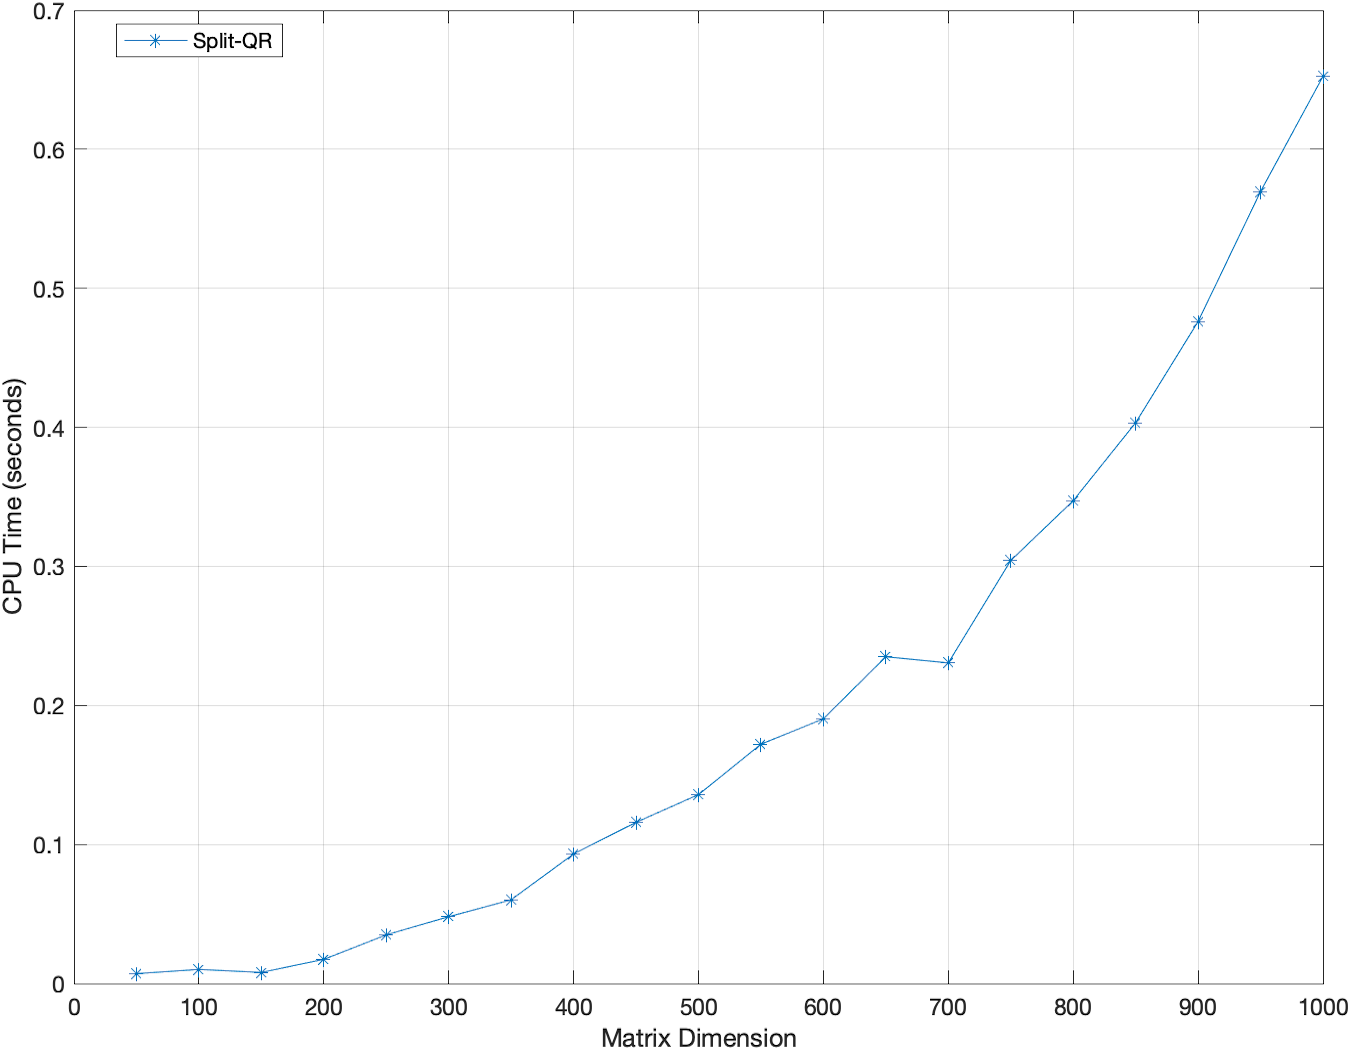
\includegraphics[width=\textwidth]{Figure_2.png} % Replace with actual filename
       % \subcaption{(a)}
    \end{minipage}
    \hfill % Add space
    \begin{minipage}[b]{0.45\textwidth}
        \centering
        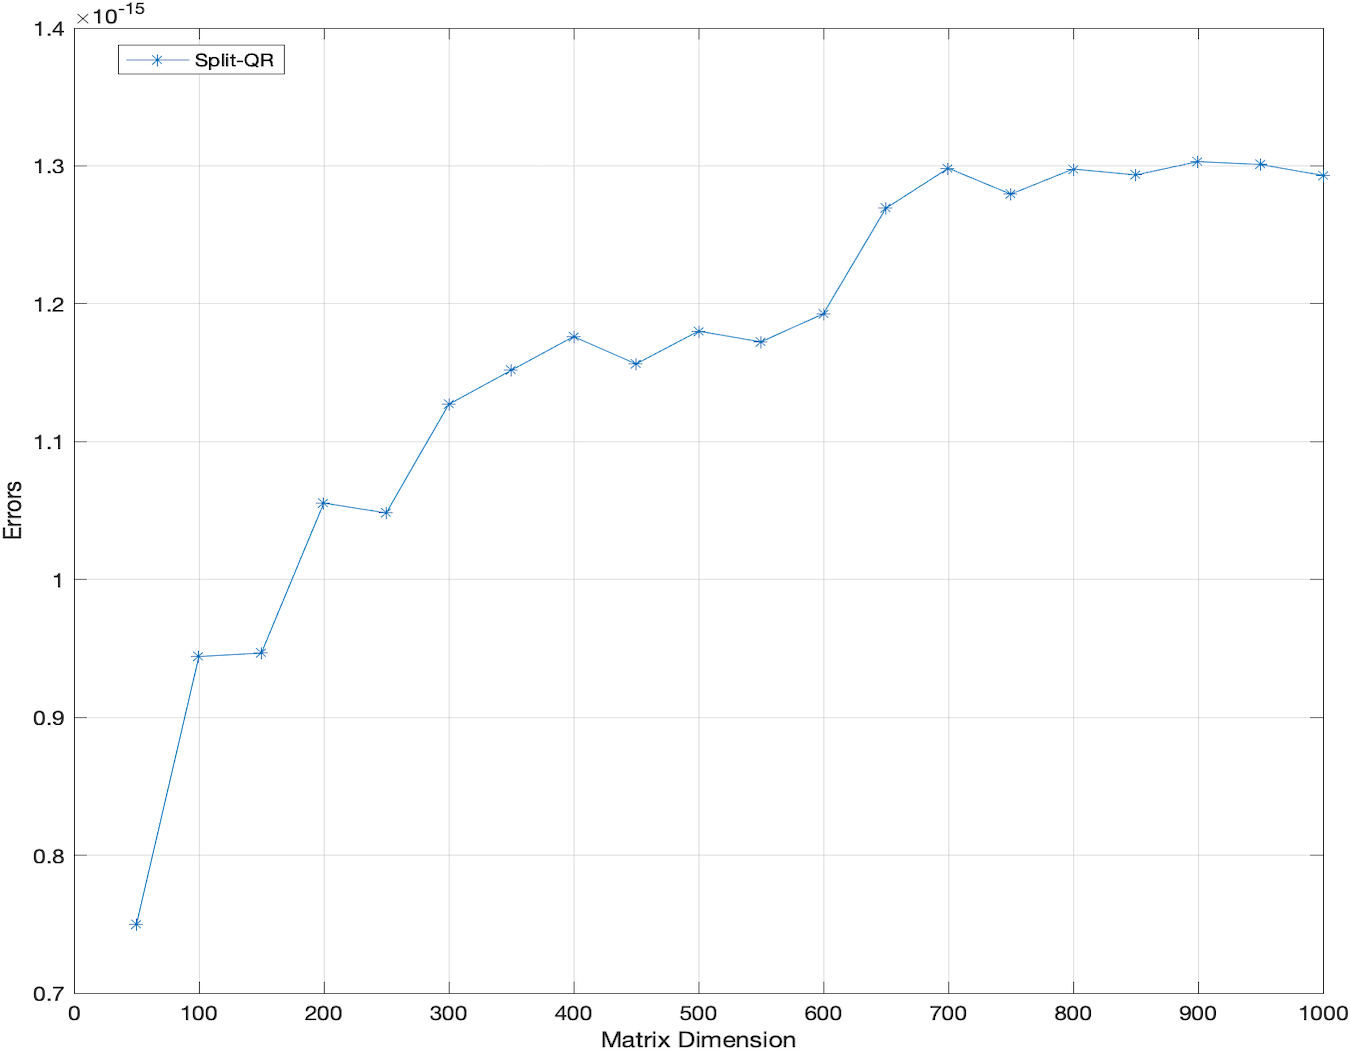
\includegraphics[width=\textwidth]{Figure_3.png} % Replace with actual filename
        % \subcaption{(b)}
    \end{minipage}
    % \captionsetup{font=footnotesize}
    \caption{ CPU Time and Error Analysis of the QR Algorithm for Split Quaternion Matrices }
     \label{fig:Figure_2}
\end{figure}

In the following, we will discuss the application of QR decomposition in solving matrix equations.
\begin{example}
Utilize the QR algorithm to solve the split quaternion matrix equation $AX = B$, where
\begin{align*}
  & A =
    \begin{bmatrix}
    -4 & -2 & -8 \\
    -2 & -2 & -5 \\
     7 & -3 & -9
    \end{bmatrix} +
    \begin{bmatrix}
    -1 & -2 &  4 \\
    -5 & -8 & -5 \\
    -4 &  0 &  6
    \end{bmatrix} i 
    + 
    \begin{bmatrix}
    -9  & -6  & -8 \\
    -2  & -10 & -5 \\
    -10 & -7  & -7
    \end{bmatrix} j +
    \begin{bmatrix}
    -8 &  9 & -3 \\
     2 & -6 &  0 \\
     8 &  0 & -5
    \end{bmatrix} k,\\
% \end{align*}
% \begin{align*}
  & B =
    \begin{bmatrix}
    -9 & -10 &  10 \\
    -1 &  10 &  6 \\
    -7 & -1  & -10
    \end{bmatrix} +
    \begin{bmatrix}
    4 &  1 & -6 \\
    4 & -6 & -3 \\
    3 &  6 &  8
    \end{bmatrix} i 
    +
    \begin{bmatrix}
     7 & 2 &  2 \\
    -2 & 9 & -4 \\
    -4 & 9 &  7
    \end{bmatrix} j +
    \begin{bmatrix}
    -1 &   1 & -3 \\
     8 &   5 & -7 \\
    -10 & -7 & -4
    \end{bmatrix} k.
\end{align*}
\end{example}  

First, using \cref{alg:QR} to perform QR decomposition on $A$ to obtain $Q$ and $R:$
\setlength{\jot}{2pt}
\setlength{\arraycolsep}{1pt}
%{\footnotesize
\begin{align*}
  Q &=
     \begin{bmatrix}
    -0.514 & -0.047 & -0.344 \\
    -0.126 & -0.411 & -0.041 \\
    -0.436 & -0.429 & -0.099
    \end{bmatrix} +
    \begin{bmatrix}
    -0.363 &  0.479 &  0.122 \\
     0.077 & -0.458 & -0.100 \\
     0.383 & -0.194 &  0.138
    \end{bmatrix} i\\
    &+ 
    \begin{bmatrix}
    -0.236 & -0.062 & -0.155 \\
    -0.105 &  0.031 &  0.403 \\
     0.262 &  0.178 & -0.296
    \end{bmatrix} j +
    \begin{bmatrix}
    -0.157 &  0.171 &  0.319 \\
    -0.250 & -0.133 &  0.577 \\
    -0.152 &  0.291 & -0.343
    \end{bmatrix} k,
    \end{align*}
    \begin{align*}
  R &=
    \begin{bmatrix}
    -3.041 & 3.419 & 10.927 \\
     0     & 6.061 & 6.456 \\
     0     & 0     & 7.714
    \end{bmatrix} +
    \begin{bmatrix}
    -1.443 & 8.617 &  1.053 \\
     0     & 1.847 & -2.947 \\
     0     & 0     & -5.025
    \end{bmatrix} i\\
    &+ 
    \begin{bmatrix}
    20.361 & 5.876  & 6.740 \\
     0     & 14.697 & 6.795 \\
     0     & 0      & 0.815
    \end{bmatrix} j +
    \begin{bmatrix}
    1.443 & -2.642 &  6.596 \\
    0     & -1.847 & -1.528 \\
    0     &  0     &  5.025
    \end{bmatrix} k.
\end{align*}
%}
Thus, the equation can be rewritten as
\begin{equation}
    QRX = B.\label{eq:example1}
\end{equation}

Since $Q$ is a unitary matrix, multiplying both sides of \eqref{eq:example1} by $Q^H$ from the left yields $RX = Q^HB\triangleq \widehat{B}$,
where
%{\footnotesize
\begin{align*}
  \widehat{B} &=
     \begin{bmatrix}
     4.981  &  6.383  &  8.076 \\
    -2.019  & -1.922  & -1.440 \\
     11.356 &  10.929 & -9.652
    \end{bmatrix} +
    \begin{bmatrix}
    -1.144 & -7.725  &  6.206 \\
     1.152 &  11.947 & -2.239 \\
    -3.761 &  0.482  & -0.749
    \end{bmatrix} i \\
    &+
    \begin{bmatrix}
    -6.136 & -7.249 & -9.693 \\
     0.310 & -4.646 &  0.574 \\
     1.391 & -2.620 & -3.994
    \end{bmatrix} j +
    \begin{bmatrix}
     11.385 & -4.261 & -2.859 \\
    -7.851  &  1.655 & -0.404 \\
    -0.653  &  6.826 &  12.841
    \end{bmatrix} k.
\end{align*}
%}
Note that $R$ is an upper triangular matrix. Thus, $RX = Q^HB\triangleq \widehat{B}$ can be solved using back substitution:
%{\footnotesize
 \begin{align*}
  X &=
    \begin{bmatrix}
    -1.082 & -0.797 &  1.407 \\
    -0.316 & -0.028 &  0.749 \\
     1.846 &  0.845 & -2.243
    \end{bmatrix} +
    \begin{bmatrix}
    -1.116 & -0.337 &  0.999 \\
    -0.423 & -0.961 &  1.907 \\
     0.349 &  1.315 & -0.403
    \end{bmatrix} i\\
    &+
    \begin{bmatrix}
    -0.456 & -0.123 &  1.793 \\
    -1.222 & -0.449 &  1.810 \\
     0.402 & -1.119 & -1.423
    \end{bmatrix} j +
    \begin{bmatrix}
     0.944 &  0.982 & -1.597 \\
     0.059 & -0.514 &  0.229 \\
    -0.989 & -0.256 &  2.156
    \end{bmatrix} k.
\end{align*}
%}
And the relative error is $\frac{\|AX - B\|_F}{\|B\|_F} = 1.2412\times 10^{-15}$.

\section{Conclusion}
\iffalse
{\color{red}We acknowledge that the split quaternion algebra does not constitute an Euclidean space, rendering traditional Givens rotations and Householder reflections inapplicable when applied to split quaternion vectors. This poses a substantial challenge for the conventional QR decomposition process for split quaternion matrices. To address this issue, by performing several permutation transformations on the rows and columns of an upper triangular matrix, we have obtained the permutation equivalence between $R$ and $R_4$: $R = P_mR_4{P_n}^T$. Based on this transformation process, we developed the Algorithm \cref{alg:Permutation}.  By analyzing the impact of the permutation matrix $P_k$ on $R$, we have proposed a more efficient optimization algorithm, Algorithm \cref{alg:Permutation Optimization}. 

Building on these findings, we introduced a special decomposition $A^\sigma = QR_4$. By utilizing the structural mapping between the real representation matrix $A^\sigma$ and the original matrix $A$, we were able to derive the QR decomposition for split quaternion matrices and subsequently propose Algorithm \cref{alg:QR}. This has filled the gap in the theory and algorithms of split quaternion QR decomposition.  Moreover, this method is broadly applicable to various decompositions, including Schur, Jordan, LU, Cholesky, and eigenvalue decompositions, etc.  Therefore, 
this new approach offers novel technical avenues for the numerical computation of split quaternion matrices.

To validate the effectiveness and superiority of the proposed algorithm, we have applied the algorithm to QR decomposition and solving matrix equation. The experimental results demonstrate that the algorithm exhibits outstanding performance, showing significant advantages in both computational efficiency and accuracy.} 
%%%%%%%%%%%%%%%%%%%%%%%%%%%%%%%%%%%%%%%%%%%%%%%%%%%%%%%%%%%%

VERSION2:\fi
In this work, we establish a critical relationship  between $R$ and $R_4$ via performing a series of permutation transformations on the rows and columns of the upper triangular matrix $R$, resulting in $R_4 = P_{2m}R{P_{2n}}^T$. By analyzing the impact of the permutation matrix $P_{2k}$ on $R$, we  propose an efficient optimization algorithm (\cref{alg:Permutation Optimization}), which will transform $R$ to $R_4$ effectively.

Based on these findings, we develop a special decomposition $A^\sigma = QR_4$. By utilizing the structural mapping between the real representation matrix $A^\sigma$ and the original matrix $A$, we were able to derive the QR decomposition for split quaternion matrices and subsequently propose \cref{alg:QR}. Upon application of this algorithm to QR decomposition and the solution of matrix equation, it exhibits outstanding performance, showing significant advantages in both computational efficiency and accuracy.

In summary, our work fills the gap in the theory and algorithms of split quaternion QR decomposition. Moreover,  the proposed new method could be used to implement various decompositions, including Schur, and eigenvalue decompositions, etc. In the future work, we will employ this method to investigate the aforementioned topics.








\iffalse
By leveraging the special decomposition $A^\sigma = QR_4$ and the unique structure of real representations for split quaternion matrices, the QR decomposition of split quaternion matrices was successfully constructed.
This paper focuses on the problem of QR decomposition for split quaternion matrices, proposing for the first time a research methodology that combines permutation operations with real representation matrices. A QR decomposition theorem suitable for split quaternion matrices is established, and a corresponding QR algorithm is constructed based on it. To validate the effectiveness and superiority of the proposed algorithm, two application examples are provided, with a systematic analysis of the algorithm's computational time consumption and relative error metrics. The experimental results demonstrate that the algorithm exhibits outstanding performance in numerical computations, showing significant advantages in both computational efficiency and accuracy. This provides new theoretical methods and technical approaches for the numerical computation of split quaternion matrices.\fi
\section*{Acknowledgment} This research is supported by \iffalse Macao Science and Technology Development Fund (No. 0013/2021/ITP),\fi  the grants from the National Natural Science Foundation of China (12371023, 12271338) and the Natural Sciences and Engineering Research Council of Canada (NSERC) (RGPIN 2020-06746). \iffalse The joint research and Development fund of Wuyi University, Hong Kong and Macao (2019WGALH20).\fi
\iffalse
{\bf Declaration of Competing Interest:} The authors declare no conflict of interest.
\\

 \fi
 \section*{Declarations}
\noindent {\bf Conflict of Interest:} The authors have not disclosed any competing interests.

\noindent {\bf Data Availability Statement:}
The data supporting the findings of this study are not publicly available due to privacy or ethical restrictions. However, interested researchers may request access to the data by contacting the corresponding author and completing any necessary data sharing agreements.
\iffalse
\section{Acknowledgments}
This research is supported by Macao Science and Technology Development Fund (No. 0013/2021/ITP),  the grants from the National Natural Science Foundation of China (12371023, 12271338) and the Natural Sciences and Engineering Research Council of Canada (NSERC) (RGPIN 2020-06746).

{\bf Data availability:} No data was used for the research described in the article.\fi
%-------------------- 参考文献 --------------------
\bibliographystyle{coam/coam} % 参考文献样式
\bibliography{references} % 文献数据库文件名

% \begin{thebibliography}{99}

% \bibitem[Abłamowicz,2020]{Abłamowicz2020}Abłamowicz R(2020)The Moore–Penrose inverse and singular value decomposition of split quaternions. Advances in Applied Clifford Algebras 30(3):33
% % \bibitem[Abłamowicz(2020)]{Abłamowicz2020} R. Abłamowicz, The Moore–Penrose inverse and singular value decomposition of split quaternions, Adv. Appl. Clifford Algebras. 33 (30) (2020) 1–20.

% \bibitem[Alagöz et al.,2012]{Yasemin2012}Alagöz Y, Oral K, Yüce S(2012)Split quaternion matrices. Miskolc Mathematical Notes 13(2):223–232
% % \bibitem[Yasemin(2012)]{Yasemin2012} Y. Alag\"oz, K. Oral, and S. Y\"uce, Split quaternion matrices, Miskolc Math. Notes 13 (2) (2012) 223–232.

% \bibitem[Cockle,1849]{Cockle1849}Cockle J(1849) LII On systems of algebra involving more than one imaginary; and on equations of the fifth degree. The London, Edinburgh, and Dublin Philosophical Magazine and Journal of Science 35(238):434-437
% % \bibitem[Cockle(1849)]{Cockle1849} J. Cockle, LII. On systems of algebra involving more than one imaginary; and on equations of the fifth degree, Phil. Mag. 35 (238) (1849) 434–437.

% \bibitem[Gogberashvili,2022]{Gog2022}Gogberashvili M(2022)(2+ 1)-Maxwell equations in split quaternions. Physics 4(1):329-363
% % \bibitem[Gog(2022)]{Gog2022} M. Gogberashvili, (2+1)-Maxwell equations in split quaternions, Phys. 4 (1) (2022) 329–363.

% \bibitem[Hasebe,2010]{Hasebe2010}Hasebe, K(2010)Split-quaternionic Hopf map, quantum Hall effect, and twistor theory. Physical Review D—Particles, Fields, Gravitation, and Cosmology 81(4):041702
% % \bibitem[Hasebe(2010)]{Hasebe2010} K. Hasebe, Split quaternionic hopf map, quantum hall effect, and twistor theory, Phys. Rev. D 81 (4) (2010) 041702.

% \bibitem[Jiang et al.,2015]{TJiang2015}Jiang T, Jiang Z, Zhang Z(2015)Algebraic techniques for diagonalization of a split quaternion matrix in split quaternionic mechanics. Journal of Mathematical Physics 56(8):083509
% % \bibitem[TJiang(2015)]{TJiang2015} T. Jiang, Z. Jiang, Z. Zhang, Algebraic techniques for diagonalization of a split quaternion matrix in split quaternion mechanics, J. Math. Phys. 56 (8) (2015) 083509.

% \bibitem[Jiang et al.,2018]{Jiang2018}Jiang T, Zhang Z, Jiang Z(2018)Algebraic techniques for eigenvalues and eigenvectors of a split quaternion matrix in split quaternionic mechanics. Computer Physics Communications 229:1-7
% % \bibitem[Jiang(2018)]{Jiang2018} T. Jiang, Z. Zhang, Z. Jiang, Algebraic techniques for eigenvalues and eigenvectors of a split quaternion matrix in split quaternionic mechanics, Comput. Phys. Comm. 229 (2018) 1–7.

% \bibitem[Jiang et al.,2018]{TJiang2018}Jiang T, Zhang Z, Jiang Z(2018)Algebraic techniques for Schrödinger equations in split quaternionic mechanics. Computers Mathematics with Applications 75(7):2217-2222
% % \bibitem[TJiang(2018)]{TJiang2018} T. Jiang, Z. Zhang, Z. Jiang, Algebraic techniques for Schrödinger equations in split quaternionic mechanics, Comput. Math. Appl. 75 (7) (2018) 2217–2222.

% \bibitem[Legrand,2022]{Le2022}Legrand EB(2022) The geometry of dissipative mechanical systems: Using Jacobi manifolds and the split quaternion algebra. Delft University of Technology
% % \bibitem[Le(2022)]{Le2022} E. Legrand, The geometry of dissipative mechanical systems: Using Jacobi manifolds and the split quaternion algebra, TU Delft, 2022.

% \bibitem[Liu \& He,2020]{Zhuo2020}Liu X, He ZH(2020)On the split quaternion matrix equation $AX= B$. Banach Journal of Mathematical Analysis 14(1):228-248
% % \bibitem[Zhuo(2020)]{Zhuo2020} X. Liu, Z. He, On the split quaternion matrix equation $AX= B$, Banach J. Math. Anal. 14 (1) (2020) 228-248.

% \bibitem[Liu \& Zhang,2020]{Yang2020}Liu X, Zhang Y(2020)Least squares \(X = {X^{\eta}}^* \) solutions to split quaternion matrix equation \(AX{A^{\eta}}^*= B\). Mathematical Methods in the Applied Sciences 43(5):2189-2201
% % \bibitem[Yang(2020)]{Yang2020} X. Liu, Y. Zhang, Least squares \(X = {X^{\eta}}^* \) solutions to split quaternion matrix equation \(AX{A^{\eta}}^*= B\), Math. Meth. Appl. Sci. 43 (5) (2020) 2189-2201.

% \bibitem[Liu \& Zhang,2019]{Xin2019}Liu X, Zhang Y(2019)Consistency of Split Quaternion Matrix Equations $AX^* - XB = CY + D$ and $X - AX^*B = CY + D$. Advances in Applied Clifford Algebras 29(4):64
% % \bibitem[Xin(2019)]{Xin2019} X. Liu and Y. Zhang. Consistency of Split Quaternion Matrix Equations $AX^* - XB = CY + D$ and $X - AX^*B = CY + D$. Advances in Applied Clifford Algebras 29 (2019) 1-20.

% \bibitem[Özdemir,2022]{Z2022}Özdemir Z(2022)A kinematic model of the Rytov’s law in the optical fiber via split quaternions: application to electromagnetic theory. The European Physical Journal Plus 137(6):651
% % \bibitem[Z(2022)]{Z2022} Z. Özdemir, A kinematic model of the Rytov’s law in the optical fiber via split quaternions: application to electromagnetic theory, Euro. Phys. J. Plus 137 (6) (2022) 1–13.

% \bibitem[Öztürk \& Özdemir,2023]{mma}Öztürk İ, Özdemir M(2023)On geometric interpretations of split quaternions. Mathematical Methods in the Applied Sciences 46(1):408-422
% % \bibitem[mma(2023)]{mma} İ. Öztürk, M. Özdemir, On geometric interpretations of split quaternions, Math. Meth. Appl. Sci. 46 (1) (2023) 408-422.

% \bibitem[Si et al.,2024]{wang}Si KW, Wang QW, Xie LM(2024)A classical system of matrix equations over the split quaternion algebra. Advances in Applied Clifford Algebras 34(5):51
% % \bibitem[wang(2024)]{wang} K.W. Si, Q.W. Wang, L.M. Xie, A classical system of matrix equations over the split quaternion algebra, Adv. Appl. Clifford Algebras. 34 (5) (2024) 51.

% \bibitem[Wang et al.,2023]{Wang2023}Wang G, Jiang T, Vasil’ev VI, Guo Z(2023)An efficient method for Maxwell’s equations with a discrete double-curl operator in split quaternionic electromagnetics. The European Physical Journal Plus 138(4):341
% % \bibitem[Wang(2023)]{Wang2023} G. Wang, T. Jiang, V.I. Vasil’ev, Z. Guo, An efficient method for Maxwell’s equations with a discrete double-curl operator in split quaternionic electromagnetics, Eur. Phys. J. Plus 341 (138) (2023) 1–6.

% \bibitem[Wang et al.2021]{Wang2021}Wang G, Jiang T, Guo Z, Zhang D(2021)A complex structure-preserving algorithm for split quaternion matrix LDU decomposition in split quaternion mechanics. Calcolo 58(3):34
% % \bibitem[Wang(2021)]{Wang2021} G. Wang, T. Jiang, Z. Guo, D. Zhang, A complex structure-preserving algorithm for split quaternion matrix LDU decomposition in split quaternion mechanics, Calcolo 58 (34) (2021) 1–15.

% \bibitem[Wang et al.,2024]{Gang2024}Wang G, Jiang T, Vasil’ev VI, Guo Z(2024)On singular value decomposition for split quaternion matrices and applications in split quaternionic mechanics. Journal of Computational and Applied Mathematics 436:115447
% % \bibitem[Gang(2024)]{Gang2024} G. Wang, T. Jiang, V. Vasil’ev, Z. Guo, On singular value decomposition for split quaternion matrices and applications in split quaternionic mechanics, J. Comput. Appl. Math. 436 (2024) 115447.

% \bibitem[Yuan et al.,2017]{yuan}Yuan SF, Wang QW, Yu YB, Tian Y(2017)On Hermitian solutions of the split quaternion matrix equation $AXB+CXD=E$. Advances in Applied Clifford Algebras 27(4):3235-3252
% % \bibitem[yuan(2017)]{yuan} S.F. Yuan, Q.W. Wang, Y. Yu, On Hermitian solutions of the split quaternion matrix equation $AXB+CXD=E$, Adv. Appl. Clifford Algebras. 27 (2017) 3235-3252.

% \bibitem[Zhang et al.,2015]{Zhang2015}Zhang Z, Jiang Z, Jiang T(2015)Algebraic methods for least squares problem in split quaternionic mechanics. Applied Mathematics and Computation 269:618-625
% % \bibitem[Zhang(2015)]{Zhang2015} Z. Zhang, Z. Jiang, T. Jiang, Algebraic methods for least squares problem in split quaternionic mechanics, Appl. Math. Comput. 269 (2015) 618–625.


% \end{thebibliography}

\end{document}